%&preformat-disser
\RequirePackage[l2tabu,orthodox]{nag} % Раскомментировав, можно в логе получать рекомендации относительно правильного использования пакетов и предупреждения об устаревших и нерекомендуемых пакетах
% Формат А4, 14pt (ГОСТ Р 7.0.11-2011, 5.3.6)
\documentclass[a4paper,14pt,oneside,openany]{memoir}

\input{common/setup}               % общие настройки шаблона
\input{common/packages}  % Пакеты общие для диссертации и автореферата
\input{Dissertation/dispackages}         % Пакеты для диссертации
\usepackage{tabu, tabulary}  %таблицы с автоматически подбирающейся шириной столбцов
\usepackage{fr-longtable}    %ради \endlasthead

\usepackage{url}
\usepackage{multirow}

% Листинги с исходным кодом программ
\usepackage{fancyvrb}
\usepackage{listings}
\lccode`\~=0\relax %Без этого хака из-за особенностей пакета listings перестают работать конструкции с \MakeLowercase и т. п. в (xe|lua)latex

% Русская традиция начертания греческих букв
\usepackage{upgreek} % прямые греческие ради русской традиции

% Микротипографика
%\ifnumequal{\value{draft}}{0}{% Только если у нас режим чистовика
%    \usepackage[final]{microtype}[2016/05/14] % улучшает представление букв и слов в строках, может помочь при наличии отдельно висящих слов
%}{}

% Отметка о версии черновика на каждой странице
% Чтобы работало надо в своей локальной копии по инструкции
% https://www.ctan.org/pkg/gitinfo2 создать небходимые файлы в папке
% ./git/hooks
% If you’re familiar with tweaking git, you can probably work it out for
% yourself. If not, I suggest you follow these steps:
% 1. First, you need a git repository and working tree. For this example,
% let’s suppose that the root of the working tree is in ~/compsci
% 2. Copy the file post-xxx-sample.txt (which is in the same folder of
% your TEX distribution as this pdf) into the git hooks directory in your
% working copy. In our example case, you should end up with a file called
% ~/compsci/.git/hooks/post-checkout
% 3. If you’re using a unix-like system, don’t forget to make the file executable.
% Just how you do this is outside the scope of this manual, but one
% possible way is with commands such as this:
% chmod g+x post-checkout.
% 4. Test your setup with “git checkout master” (or another suitable branch
% name). This should generate copies of gitHeadInfo.gin in the directories
% you intended.
% 5. Now make two more copies of this file in the same directory (hooks),
% calling them post-commit and post-merge, and you’re done. As before,
% users of unix-like systems should ensure these files are marked as
% executable.
\ifnumequal{\value{draft}}{1}{% Черновик
   \IfFileExists{.git/gitHeadInfo.gin}{                                        
      \usepackage[mark,pcount]{gitinfo2}
      \renewcommand{\gitMark}{rev.\gitAbbrevHash\quad\gitCommitterEmail\quad\gitAuthorIsoDate}
      \renewcommand{\gitMarkFormat}{\color{Gray}\small\bfseries}
   }{}
}{}        % Пакеты для специфических пользовательских задач

\input{Dissertation/setup}               % Упрощённые настройки шаблона

\input{Dissertation/preamblenames}       % Переопределение именований, чтобы можно было и в преамбуле использовать
\input{common/newnames}  % Новые переменные, которые могут использоваться во всём проекте

%%% Основные сведения %%%
\newcommand{\thesisAuthor}             % Диссертация, ФИО автора
{%
    \texorpdfstring{% \texorpdfstring takes two arguments and uses the first for (La)TeX and the second for pdf
        Демчев Денис Михайлович% так будет отображаться на титульном листе или в тексте, где будет использоваться переменная
    }{%
        Демчев Денис Михайлович% эта запись для свойств pdf-файла. В таком виде, если pdf будет обработан программами для сбора библиографических сведений, будет правильно представлена фамилия.
    }%
}
\newcommand{\thesisAuthorShort}        % Диссертация, ФИО автора инициалами
{Д.М.~Демчев}

\newcommand{\thesisUdk}                % Диссертация, УДК
{551.326.14+528.8.044.2}
\newcommand{\thesisTitle}              % Диссертация, название
{\texorpdfstring{\MakeUppercase{Мониторинг дрейфа льда на основе спутниковых данных активной радиолокации в Арктике}}{Мониторинг дрейфа льда на основе спутниквых SAR"--~ данных в Арктике}}
\newcommand{\thesisSpecialtyNumber}    % Диссертация, специальность, номер
{\texorpdfstring{25.00.28}{25.00.28}}
\newcommand{\thesisSpecialtyTitle}     % Диссертация, специальность, название
{\texorpdfstring{Океанология}{Океанология}}
\newcommand{\thesisDegree}             % Диссертация, ученая степень
{\todo{кандидата технических наук}}
\newcommand{\thesisDegreeShort}        % Диссертация, ученая степень, краткая запись
{\todo{канд. физ.-мат. наук}}
\newcommand{\thesisCity}               % Диссертация, город написания диссертации
{Санкт-Петербург}
\newcommand{\thesisYear}               % Диссертация, год написания диссертации
{2017}
\newcommand{\thesisOrganization}       % Диссертация, организация
{МЕЖДУНАРОДНЫЙ ЦЕНТР ПО ОКРУЖАЮЩЕЙ СРЕДЕ И ДИСТАНЦИОННОМУ ЗОНДИРОВАНИЮ имени НАНСЕНА}
\newcommand{\thesisOrganizationShort}  % Диссертация, краткое название организации для доклада
{\todo{Фонд <<Нансен-Центр>>}}

\newcommand{\thesisInOrganization}     % Диссертация, организация в предложном падеже: Работа выполнена в ...
{\todo{МЕЖДУНАРОДНОМ ЦЕНТРЕ ПО ОКРУЖАЮЩЕЙ СРЕДЕ И ДИСТАНЦИОННОМУ ЗОНДИРОВАНИЮ имени НАНСЕНА}}

\newcommand{\supervisorFio}            % Научный руководитель, ФИО
{\todo{Фамилия Имя Отчество}}
\newcommand{\supervisorRegalia}        % Научный руководитель, регалии
{\todo{уч. степень, уч. звание}}
\newcommand{\supervisorFioShort}       % Научный руководитель, ФИО
{\todo{И.О.~Фамилия}}
\newcommand{\supervisorRegaliaShort}   % Научный руководитель, регалии
{\todo{уч.~ст.,~уч.~зв.}}


\newcommand{\opponentOneFio}           % Оппонент 1, ФИО
{\todo{Фамилия Имя Отчество}}
\newcommand{\opponentOneRegalia}       % Оппонент 1, регалии
{\todo{доктор физико-математических наук, профессор}}
\newcommand{\opponentOneJobPlace}      % Оппонент 1, место работы
{\todo{Не очень длинное название для места работы}}
\newcommand{\opponentOneJobPost}       % Оппонент 1, должность
{\todo{старший научный сотрудник}}

\newcommand{\opponentTwoFio}           % Оппонент 2, ФИО
{\todo{Фамилия Имя Отчество}}
\newcommand{\opponentTwoRegalia}       % Оппонент 2, регалии
{\todo{кандидат физико-математических наук}}
\newcommand{\opponentTwoJobPlace}      % Оппонент 2, место работы
{\todo{Основное место работы c длинным длинным длинным длинным названием}}
\newcommand{\opponentTwoJobPost}       % Оппонент 2, должность
{\todo{старший научный сотрудник}}

\newcommand{\leadingOrganizationTitle} % Ведущая организация, дополнительные строки
{\todo{Федеральное государственное бюджетное образовательное учреждение высшего профессионального образования с~длинным длинным длинным длинным названием}}

\newcommand{\defenseDate}              % Защита, дата
{\todo{DD mmmmmmmm YYYY~г.~в~XX часов}}
\newcommand{\defenseCouncilNumber}     % Защита, номер диссертационного совета
{\todo{Д\,123.456.78}}
\newcommand{\defenseCouncilTitle}      % Защита, учреждение диссертационного совета
{\todo{Название учреждения}}
\newcommand{\defenseCouncilAddress}    % Защита, адрес учреждение диссертационного совета
{\todo{Адрес}}
\newcommand{\defenseCouncilPhone}      % Телефон для справок
{\todo{+7~(0000)~00-00-00}}

\newcommand{\defenseSecretaryFio}      % Секретарь диссертационного совета, ФИО
{\todo{Фамилия Имя Отчество}}
\newcommand{\defenseSecretaryRegalia}  % Секретарь диссертационного совета, регалии
{\todo{д-р~физ.-мат. наук}}            % Для сокращений есть ГОСТы, например: ГОСТ Р 7.0.12-2011 + http://base.garant.ru/179724/#block_30000

\newcommand{\synopsisLibrary}          % Автореферат, название библиотеки
{\todo{Название библиотеки}}
\newcommand{\synopsisDate}             % Автореферат, дата рассылки
{\todo{DD mmmmmmmm YYYY года}}

% To avoid conflict with beamer class use \providecommand
\providecommand{\keywords}%            % Ключевые слова для метаданных PDF диссертации и автореферата
{}      % Основные сведения
\input{common/styles}    % Стили общие для диссертации и автореферата
\input{Dissertation/disstyles}           % Стили для диссертации
\input{Dissertation/userstyles}          % Стили для специфических пользовательских задач
\input{biblio/bibliopreamble}% Настройки библиографии из внешнего файла (там же выбор: встроенная или на основе biblatex)

\input{Dissertation/inclusioncontrol}    % Управление компиляцией отдельных частей диссертации

\begin{document}

\input{common/renames}                   % Переопределение именований

% Структура диссертации (ГОСТ Р 7.0.11-2011, 4)
% Титульный лист (ГОСТ Р 7.0.11-2001, 5.1)
\thispagestyle{empty}%
\begin{center}%
\MakeUppercase{\thesisOrganization}
\end{center}%
%
\vspace{0pt plus4fill} %число перед fill = кратность относительно некоторого расстояния fill, кусками которого заполнены пустые места
\IfFileExists{images/logo.pdf}{
  \begin{minipage}[b]{0.499\linewidth}
    \begin{flushleft}%
      
\includegraphics[height=3.5cm]{logo}
    \end{flushleft}
  \end{minipage}
  \begin{minipage}[b]{0.499\linewidth}
    \begin{flushright}%
      На правах рукописи\\
       \textsl {УДК \thesisUdk}
    \end{flushright}%
  \end{minipage}
}{
\begin{flushright}%
На правах рукописи

%\textsl {УДК \thesisUdk}
\end{flushright}%
}
%
\vspace{0pt plus6fill} %число перед fill = кратность относительно некоторого расстояния fill, кусками которого заполнены пустые места
\begin{center}%
{\large \thesisAuthor}
\end{center}%
%
\vspace{0pt plus1fill} %число перед fill = кратность относительно некоторого расстояния fill, кусками которого заполнены пустые места
\begin{center}%
\textbf {\large \thesisTitle}

\vspace{0pt plus2fill} %число перед fill = кратность относительно некоторого расстояния fill, кусками которого заполнены пустые места
{%\small
Специальность \thesisSpecialtyNumber~---

<<\thesisSpecialtyTitle>>
}

\vspace{0pt plus2fill} %число перед fill = кратность относительно некоторого расстояния fill, кусками которого заполнены пустые места
Диссертация на соискание учёной степени

\thesisDegree
\end{center}%
%
\vspace{0pt plus4fill} %число перед fill = кратность относительно некоторого расстояния fill, кусками которого заполнены пустые места
\begin{flushright}%
Научный руководитель:

\supervisorRegalia

\supervisorFio
\end{flushright}%
%
\vspace{0pt plus4fill} %число перед fill = кратность относительно некоторого расстояния fill, кусками которого заполнены пустые места
\begin{center}%
{\thesisCity~--- \thesisYear}
\end{center}%
\newpage
           % Титульный лист
\include{Dissertation/contents}        % Оглавление
\include{Dissertation/introduction}    % Введение
\chapter{Оформление различных элементов} \label{chapt1}

\section{Форматирование текста} \label{sect1_1}

Мы можем сделать \textbf{жирный текст} и \textit{курсив}.

%\newpage
%============================================================================================================================

\section{Ссылки} \label{sect1_2}
Сошлёмся на библиографию.
%Одна ссылка: \cite[с.~54]{Sokolov}\cite[с.~36]{Gaidaenko}.
%Две ссылки: \cite{Sokolov,Gaidaenko}.
%Много ссылок: %\cite[с.~54]{Lermontov,Management,Borozda} % такой «фокус» вызывает biblatex warning относительно опции sortcites, потому что неясно, к какому источнику относится уточнение о страницах, а bibtex об этой проблеме даже не предупреждает
%\cite{Lermontov,Management,Borozda,Marketing,Constitution,FamilyCode,Gost.7.0.53,Razumovski,Lagkueva,Pokrovski,Sirotko,Lukina,Methodology,Encyclopedia,Nasirova,Berestova,Kriger}.
И ещё немного ссылок:
%\cite{Article,Book,Booklet,Conference,Inbook,Incollection,Manual,Mastersthesis,Misc,Phdthesis,Proceedings,Techreport,Unpublished}.
%\cite{medvedev2006jelektronnye, CEAT:CEAT581, doi:10.1080/01932691.2010.513279,Gosele1999161,Li2007StressAnalysis, Shoji199895,test:eisner-sample,AB_patent_Pomerantz_1968,iofis_patent1960}

%Попытка реализовать несколько ссылок на конкретные страницы для стандартной реализации:[\citenum{Sokolov}, с.~54; \citenum{Gaidaenko}, с.~36].

%Несколько источников мультицитата \cites[vii--x, 5, 7]{Sokolov}[v--x, 25, 526]{Gaidaenko} поехали дальше

Ссылки на собственные работы:~\cite{vakbib1, confbib1}

Сошлёмся на приложения: Приложение \ref{AppendixA}, Приложение \ref{AppendixB2}.

Сошлёмся на формулу: формула \eqref{eq:equation1}.

Сошлёмся на изображение: рисунок \ref{img:knuth}.

%\newpage
%============================================================================================================================

\section{Формулы} \label{sect1_3}

Благодаря пакету \textit{icomma}, \LaTeX~одинаково хорошо воспринимает в качестве десятичного разделителя и запятую ($3,1415$), и точку ($3.1415$).

\subsection{Ненумерованные одиночные формулы} \label{subsect1_3_1}

Вот так может выглядеть формула, которую необходимо вставить в строку по тексту: $x \approx \sin x$ при $x \to 0$.

А вот так выглядит ненумерованая отдельностоящая формула c подстрочными и надстрочными индексами:
\[
(x_1+x_2)^2 = x_1^2 + 2 x_1 x_2 + x_2^2
\]

При использовании дробей формулы могут получаться очень высокие:
\[
  \frac{1}{\sqrt{2}+
  \displaystyle\frac{1}{\sqrt{2}+
  \displaystyle\frac{1}{\sqrt{2}+\cdots}}}
\]

В формулах можно использовать греческие буквы:
\[
\alpha\beta\gamma\delta\epsilon\varepsilon\zeta\eta\theta\vartheta\iota\kappa\lambda\\mu\nu\xi\pi\varpi\rho\varrho\sigma\varsigma\tau\upsilon\phi\varphi\chi\psi\omega\Gamma\Delta\Theta\Lambda\Xi\Pi\Sigma\Upsilon\Phi\Psi\Omega
\]

\def\slantfrac#1#2{ \hspace{3pt}\!^{#1}\!\!\hspace{1pt}/
  \hspace{2pt}\!\!_{#2}\!\hspace{3pt}
} %Макрос для красивых дробей в строчку (например, 1/2)
Для красивых дробей (например, в индексах) можно добавить макрос
\verb+\slantfrac+ и писать $\slantfrac{1}{2}$ вместо $1/2$.
%\newpage
%============================================================================================================================

\subsection{Ненумерованные многострочные формулы} \label{subsect1_3_2}

Вот так можно написать две формулы, не нумеруя их, чтобы знаки равно были строго друг под другом:
\begin{align}
  f_W & =  \min \left( 1, \max \left( 0, \frac{W_{soil} / W_{max}}{W_{crit}} \right)  \right), \nonumber \\
  f_T & =  \min \left( 1, \max \left( 0, \frac{T_s / T_{melt}}{T_{crit}} \right)  \right), \nonumber
\end{align}

Выровнять систему ещё и по переменной $ x $ можно, используя окружение \verb|alignedat| из пакета \verb|amsmath|. Вот так: 
\[
    |x| = \left\{
    \begin{alignedat}{2}
        &&x, \quad &\text{eсли } x\geqslant 0 \\
        &-&x, \quad & \text{eсли } x<0
    \end{alignedat}
    \right.
\]
Здесь первый амперсанд (в исходном \LaTeX\ описании формулы) означает выравнивание по~левому краю, второй "--- по~$ x $, а~третий "--- по~слову <<если>>. Команда \verb|\quad| делает большой горизонтальный пробел.

Ещё вариант:
\[
    |x|=
    \begin{cases}
    \phantom{-}x, \text{если } x \geqslant 0 \\
    -x, \text{если } x<0
    \end{cases}
\]

Кроме того, для  нумерованых формул \verb|alignedat|  делает вертикальное
выравнивание номера формулы по центру формулы. Например,  выравнивание компонент вектора:
\begin{equation}
 \label{eq:2p3}
 \begin{alignedat}{2}
{\mathbf{N}}_{o1n}^{(j)} = \,{\sin} \phi\,n\!\left(n+1\right)
         {\sin}\theta\,
         \pi_n\!\left({\cos} \theta\right)
         \frac{
               z_n^{(j)}\!\left( \rho \right)
              }{\rho}\,
           &{\boldsymbol{\hat{\mathrm e}}}_{r}\,+   \\
+\,
{\sin} \phi\,
         \tau_n\!\left({\cos} \theta\right)
         \frac{
            \left[\rho z_n^{(j)}\!\left( \rho \right)\right]^{\prime}
              }{\rho}\,
            &{\boldsymbol{\hat{\mathrm e}}}_{\theta}\,+   \\
+\,
{\cos} \phi\,
         \pi_n\!\left({\cos} \theta\right)
         \frac{
            \left[\rho z_n^{(j)}\!\left( \rho \right)\right]^{\prime}
              }{\rho}\,
            &{\boldsymbol{\hat{\mathrm e}}}_{\phi}\:.
\end{alignedat}
\end{equation}

Ещё об отступах. Иногда для лучшей <<читаемости>> формул полезно
немного исправить стандартные интервалы \LaTeX\ с учётом логической
структуры самой формулы. Например в формуле~\ref{eq:2p3} добавлен
небольшой отступ \verb+\,+ между основными сомножителями, ниже
результат применения всех вариантов отступа:
\begin{align*}
\backslash! &\quad f(x) = x^2\! +3x\! +2 \\
  \mbox{по-умолчанию} &\quad f(x) = x^2+3x+2 \\
\backslash, &\quad f(x) = x^2\, +3x\, +2 \\
\backslash{:} &\quad f(x) = x^2\: +3x\: +2 \\
\backslash; &\quad f(x) = x^2\; +3x\; +2 \\
\backslash \mbox{space} &\quad f(x) = x^2\ +3x\ +2 \\
\backslash \mbox{quad} &\quad f(x) = x^2\quad +3x\quad +2 \\
\backslash \mbox{qquad} &\quad f(x) = x^2\qquad +3x\qquad +2
\end{align*}


Можно использовать разные математические алфавиты:
\begin{align}
\mathcal{ABCDEFGHIJKLMNOPQRSTUVWXYZ} \nonumber \\
\mathfrak{ABCDEFGHIJKLMNOPQRSTUVWXYZ} \nonumber \\
\mathbb{ABCDEFGHIJKLMNOPQRSTUVWXYZ} \nonumber
\end{align}

Посмотрим на систему уравнений на примере аттрактора Лоренца:

\[ 
\left\{
  \begin{array}{rl}
    \dot x = & \sigma (y-x) \\
    \dot y = & x (r - z) - y \\
    \dot z = & xy - bz
  \end{array}
\right.
\]

А для вёрстки матриц удобно использовать многоточия:
\[ 
\left(
  \begin{array}{ccc}
  	a_{11} & \ldots & a_{1n} \\
  	\vdots & \ddots & \vdots \\
  	a_{n1} & \ldots & a_{nn} \\
  \end{array}
\right)
\]


%\newpage
%============================================================================================================================
\subsection{Нумерованные формулы} \label{subsect1_3_3}

А вот так пишется нумерованая формула:
\begin{equation}
  \label{eq:equation1}
  e = \lim_{n \to \infty} \left( 1+\frac{1}{n} \right) ^n
\end{equation}

Нумерованых формул может быть несколько:
\begin{equation}
  \label{eq:equation2}
  \lim_{n \to \infty} \sum_{k=1}^n \frac{1}{k^2} = \frac{\pi^2}{6}
\end{equation}

Впоследствии на формулы (\ref{eq:equation1}) и (\ref{eq:equation2}) можно ссылаться.

Сделать так, чтобы номер формулы стоял напротив средней строки, можно, используя окружение \verb|multlined| (пакет \verb|mathtools|) вместо \verb|multline| внутри окружения \verb|equation|. Вот так:
\begin{equation} % \tag{S} % tag - вписывает свой текст 
  \label{eq:equation3}
    \begin{multlined}
        1+ 2+3+4+5+6+7+\dots + \\ 
        + 50+51+52+53+54+55+56+57 + \dots + \\ 
        + 96+97+98+99+100=5050 
    \end{multlined}
\end{equation}

Используя команду \verb|\labelcref| из пакета \verb|cleveref|, можно
красиво ссылаться сразу на несколько формул
(\labelcref{eq:equation1,eq:equation3,eq:equation2}), даже перепутав
порядок ссылок \verb|(\labelcref{eq:equation1,eq:equation3,eq:equation2})|.

           % Глава 1
\chapter{Восстановление полей дрейфа льда методом прослеживание особых точек на~SAR"~изображениях} \label{chapt2}

\section{Одиночное изображение} \label{sect2_1}

\begin{figure}[ht] 
  \centering
  \includegraphics [scale=0.27] {latex}
  \caption{TeX.}
  \label{img:latex}
\end{figure}

%\newpage
%============================================================================================================================
\section{Длинное название параграфа, в котором мы узнаём как сделать две картинки с~общим номером и названием} \label{sect2_2}

А это две картинки под общим номером и названием:
\begin{figure}[ht]
  \begin{minipage}[ht]{0.49\linewidth}\centering
    \includegraphics[width=0.5\linewidth]{knuth1} \\ а)
  \end{minipage}
  \hfill
  \begin{minipage}[ht]{0.49\linewidth}\centering
    \includegraphics[width=0.5\linewidth]{knuth2} \\ б)
  \end{minipage}
  \caption{Очень длинная подпись к изображению, на котором представлены две фотографии Дональда Кнута}
  \label{img:knuth}  
\end{figure}

Те~же~две картинки под~общим номером и~названием, но с автоматизированной нумерацией подрисунков:
\begin{figure}[ht]
    {\centering
        \hfill
        \subbottom[List-of-Figures entry][Первый подрисунок\label{img:knuth_2_1}]{%
            \includegraphics[width=0.25\linewidth]{knuth1}}
        \hfill
        \subbottom[\label{img:knuth_2_2}]{%
            \includegraphics[width=0.25\linewidth]{knuth2}}
        \hfill
        \subbottom[Третий подрисунок]{%
            \includegraphics[width=0.3\linewidth]{example-image-c}}
        \hfill
    }
    \legend{Подрисуночный текст, описывающий обозначения, например. Согласно
    ГОСТ 2.105, пункт 4.3.1, располагается перед наименованием рисунка.}
    \caption[Этот текст попадает в названия рисунков в списке рисунков]{Очень
    длинная подпись к второму изображению, на котором представлены две
    фотографии Дональда Кнута}
    \label{img:knuth_2}
\end{figure}

На рисунке~\ref{img:knuth_2_1} показан Дональд Кнут без головного убора. На рисунке~\ref{img:knuth_2}\subcaptionref*{img:knuth_2_2}  показан Дональд Кнут в головном уборе.

%\newpage
%============================================================================================================================
\section{Пример вёрстки списков} \label{sect2_3}

\noindent Нумерованный список:
\begin{enumerate}
  \item Первый пункт.
  \item Второй пункт.
  \item Третий пункт.
\end{enumerate}

\noindent Маркированный список:
\begin{itemize}
  \item Первый пункт.
  \item Второй пункт.
  \item Третий пункт.
\end{itemize}

\noindent Вложенные списки:
\begin{itemize}
  \item Имеется маркированный список.
  \begin{enumerate}
    \item В нём лежит нумерованный список,
    \item в котором
    \begin{itemize}
      \item лежит ещё один маркированный список.
    \end{itemize}    
  \end{enumerate}
\end{itemize}

\noindent Нумерованные вложенные списки:
\begin{enumerate}
  \item Первый пункт.
  \item Второй пункт.
  \item Вообще, по ГОСТ 2.105 первый уровень нумерации
  (при необходимости ссылки в тексте документа на одно из перечислений)
  идёт буквами русского или латинского алфавитов,
  а второй "--- цифрами со скобками.
  Здесь отходим от ГОСТ.
    \begin{enumerate}
      \item в нём лежит нумерованный список,
      \item в котором
        \begin{enumerate}
          \item ещё один нумерованный список,
          \item третий уровень нумерации не нормирован ГОСТ 2.105;
          \item обращаем внимание на строчность букв,
          \item в этом списке
          \begin{itemize}
            \item лежит ещё один маркированный список.
          \end{itemize}    
        \end{enumerate}

    \end{enumerate}

  \item Четвёртый пункт.
\end{enumerate}

\section{Традиции русского набора}

Много полезных советов приведено в материале
<<\href{http://www.dropbox.com/s/x4hajy4pkw3wdql/wholesome-typesetting.pdf?dl=1\&pv=1}{Краткий курс благородного набора}>> (автор А.\:В.~Костырка).
Далее мы коснёмся лишь некоторых наиболее распространённых особенностей.

\subsection{Пробелы}

В~русском наборе принято:
\begin{itemize}
    \item единицы измерения, знак процента отделять пробелами от~числа: 10~кВт, 15~\% (согласно ГОСТ 8.417, раздел 8);
    \item $\tg 20^\circ$, но: 20~${}^\circ$C (согласно ГОСТ 8.417, раздел 8);
    \item знак номера, параграфа отделять от~числа: №~5, \S~8;
    \item стандартные сокращения: т.\:е., и~т.\:д., и~т.\:п.;
    \item неразрывные пробелы в~предложениях.
\end{itemize}

\subsection{Математические знаки и символы}

Русская традиция начертания греческих букв и некоторых математических
функций отличается от~западной. Это исправляется серией
\verb|\renewcommand|.
\begin{itemize}
%Все \original... команды заранее, ради этого примера, определены в Dissertation\userstyles.tex
    \item[До:] \( \originalepsilon \originalge \originalphi\),
    \(\originalphi \originalleq \originalepsilon\),
    \(\originalkappa \in \originalemptyset\),
    \(\originaltan\),
    \(\originalcot\),
    \(\originalcsc\).
    \item[После:] \( \epsilon \ge \phi\),
    \(\phi \leq \epsilon\),
    \(\kappa \in \emptyset\),
    \(\tan\),
    \(\cot\),
    \(\csc\).
\end{itemize}

Кроме того, принято набирать греческие буквы вертикальными, что
решается подключением пакета \verb|upgreek| (см. закомментированный
блок в~\verb|userpackages.tex|) и~аналогичным переопределением в
преамбуле (см.~закомментированный блок в \verb|userstyles.tex|). В
этом шаблоне такие переопределения уже включены.

Знаки математических операций принято переносить. Пример переноса
в~формуле \eqref{eq:equation3}.

\subsection{Кавычки}
В английском языке приняты одинарные и двойные кавычки в~виде ‘...’ и~“...”. В России приняты французские («...») и~немецкие („...“) кавычки (они называются «ёлочки» и~«лапки», соответственно). <<Лапки>> обычно используются внутри ,,ёлочек``, например, <<... наш гордый ,,Варяг``...>>.

Французкие левые и правые кавычки набираются
как лигатуры \verb|<<| и \verb|>>|, а~немецкие левые и правые кавычки набираются как лигатуры \verb|,,| и \verb|‘‘| (\verb|``|).

Вместо лигатур или команд с~активным символом "\ можно использовать команды \verb|\glqq| и \verb|\grqq| для набора немецких кавычек и команды \verb|\flqq| и \verb|\frqq| для набора французских кавычек. Они определены в пакете \verb|babel|.

\subsection{Тире}
%  babel+pdflatex по умолчанию, в polyglossia надо включать опцией (и перекомпилировать с удалением временных файлов)
Команда \verb|"---| используется для печати тире в тексте. Оно несколько короче английского длинного тире. Кроме того, команда задаёт небольшую жёсткую отбивку от слова, стоящего перед тире. При этом, само тире не отрывается от~слова. После тире следует такая же отбивка от текста, как и перед тире. При наборе текста между словом и командой, за которым она следует, должен стоять пробел.

В составных словах, таких, как <<Закон Менделеева"--~Клапейрона>>, для печати тире надо использовать команду \verb|"--~|. Она ставит более короткое, по~сравнению с~английским, тире и позволяет делать переносы во втором слове. При~наборе текста команда \verb|"--~| не отделяется пробелом от слова, за которым она следует (\verb|Менделеева"--~|). Следующее за командой слово может быть  отделено от~неё пробелом или перенесено на другую строку.

Если прямая речь начинается с~абзаца, то перед началом её печатается тире командой
\verb|"--*|. Она печатает русское тире и жёсткую отбивку нужной величины перед текстом.

\subsection{Дефисы и переносы слов}
%  babel+pdflatex по умолчанию, в polyglossia надо включать опцией (и перекомпилировать с удалением временных файлов)
Для печати дефиса в~составных словах введены две команды. Команда~\verb|"~| печатает дефис и~запрещает делать переносы в~самих словах, а~команда \verb|"=| печатает дефис, оставляя \TeX ’у право делать переносы в~самих словах.

В отличие от команды \verb|\-|, команда \verb|"-| задаёт место в~слове, где можно делать перенос, не~запрещая переносы и~в~других местах слова.

Команда \verb|""| задаёт место в~слове, где можно делать перенос, причём дефис при~переносе в~этом месте не~ставится.

Команда \verb|",| вставляет небольшой пробел после инициалов с~правом переноса в~фамилии.

\section{Текст из панграмм и формул}

Любя, съешь щипцы, "--- вздохнёт мэр, "--- кайф жгуч. Шеф взъярён тчк щипцы с~эхом гудбай Жюль. Эй, жлоб! Где туз? Прячь юных съёмщиц в~шкаф. Экс-граф? Плюш изъят. Бьём чуждый цен хвощ! Эх, чужак! Общий съём цен шляп (юфть) "--- вдрызг! Любя, съешь щипцы, "--- вздохнёт мэр, "--- кайф жгуч. Шеф взъярён тчк щипцы с~эхом гудбай Жюль. Эй, жлоб! Где туз? Прячь юных съёмщиц в~шкаф. Экс-граф? Плюш изъят. Бьём чуждый цен хвощ! Эх, чужак! Общий съём цен шляп (юфть) "--- вдрызг! Любя, съешь щипцы, "--- вздохнёт мэр, "--- кайф жгуч. Шеф взъярён тчк щипцы с~эхом гудбай Жюль. Эй, жлоб! Где туз? Прячь юных съёмщиц в~шкаф. Экс-граф? Плюш изъят. Бьём чуждый цен хвощ! Эх, чужак! Общий съём цен шляп (юфть) "--- вдрызг! Любя, съешь щипцы, "--- вздохнёт мэр, "--- кайф жгуч. Шеф взъярён тчк щипцы с~эхом гудбай Жюль. Эй, жлоб! Где туз? Прячь юных съёмщиц в~шкаф. Экс-граф? Плюш изъят. Бьём чуждый цен хвощ! Эх, чужак! Общий съём цен шляп (юфть) "--- вдрызг! Любя, съешь щипцы, "--- вздохнёт мэр, "--- кайф жгуч. Шеф взъярён тчк щипцы с~эхом гудбай Жюль. Эй, жлоб! Где туз? Прячь юных съёмщиц в~шкаф. Экс-граф? Плюш изъят. Бьём чуждый цен хвощ! Эх, чужак! Общий съём цен шляп (юфть) "--- вдрызг! Любя, съешь щипцы, "--- вздохнёт мэр, "--- кайф жгуч. Шеф взъярён тчк щипцы с~эхом гудбай Жюль. Эй, жлоб! Где туз? Прячь юных съёмщиц в~шкаф. Экс-граф? Плюш изъят. Бьём чуждый цен хвощ! Эх, чужак! Общий съём цен шляп (юфть) "--- вдрызг! Любя, съешь щипцы, "--- вздохнёт мэр, "--- кайф жгуч. Шеф взъярён тчк щипцы с~эхом гудбай Жюль. Эй, жлоб! Где туз? Прячь юных съёмщиц в~шкаф. Экс-граф? Плюш изъят. Бьём чуждый цен хвощ! Эх, чужак! Общий съём цен шляп (юфть) "--- вдрызг! Любя, съешь щипцы, "--- вздохнёт мэр, "--- кайф жгуч. Шеф взъярён тчк щипцы с~эхом гудбай Жюль. Эй, жлоб! Где туз? Прячь юных съёмщиц в~шкаф. Экс-граф? Плюш изъят. Бьём чуждый цен хвощ! Эх, чужак! Общий съём цен шляп (юфть) "--- вдрызг! Любя, съешь щипцы, "--- вздохнёт мэр, "--- кайф жгуч. Шеф взъярён тчк щипцы с~эхом гудбай Жюль. Эй, жлоб! Где туз? Прячь юных съёмщиц в~шкаф. Экс-граф? Плюш изъят. Бьём чуждый цен хвощ! Эх, чужак! Общий съём цен шляп (юфть) "--- вдрызг! Любя, съешь щипцы, "--- вздохнёт мэр, "--- кайф жгуч. Шеф взъярён тчк щипцы с~эхом гудбай Жюль. Эй, жлоб! Где туз? Прячь юных съёмщиц в~шкаф. Экс-граф? Плюш изъят. Бьём чуждый цен хвощ! Эх, чужак! Общий съём цен шляп (юфть) "--- вдрызг! Любя, съешь щипцы, "--- вздохнёт мэр, "--- кайф жгуч. Шеф взъярён тчк щипцы с~эхом гудбай Жюль. Эй, жлоб! Где туз? Прячь юных съёмщиц в~шкаф. Экс-граф? Плюш изъят. Бьём чуждый цен хвощ! Эх, чужак! Общий съём цен шляп (юфть) "--- вдрызг!Любя, съешь щипцы, "--- вздохнёт мэр, "--- кайф жгуч. Шеф взъярён тчк щипцы с~эхом гудбай Жюль. Эй, жлоб! Где туз? Прячь юных съёмщиц в~шкаф. Экс-граф? Плюш изъят. Бьём чуждый цен хвощ! Эх, чужак! Общий съём цен

Ку кхоро адолэжкэнс волуптариа хаж, вим граэко ыкчпэтында ты. Граэкы жэмпэр льюкяльиюч квуй ку, аэквюы продыжщэт хаж нэ. Вим ку магна пырикульа, но квюандо пожйдонёюм про. Квуй ат рыквюы ёнэрмйщ. Выро аккузата вим нэ.
\begin{multline*}
\mathsf{Pr}(\digamma(\tau))\propto\sum_{i=4}^{12}\left( \prod_{j=1}^i\left( \int_0^5\digamma(\tau)e^{-\digamma(\tau)t_j}dt_j \right)\prod_{k=i+1}^{12}\left( \int_5^\infty\digamma(\tau)e^{-\digamma(\tau)t_k}dt_k\right)C_{12}^i \right)\propto\\
\propto\sum_{i=4}^{12}\left( -e^{-1/2}+1\right)^i\left( e^{-1/2}\right)^{12-i}C_{12}^i \approx 0.7605,\quad \forall\tau\neq\overline{\tau}
\end{multline*}
Квуй ыёюз омниюм йн. Экз алёквюам кончюлату квуй, ты альяквюам ёнвидюнт пэр. Зыд нэ коммодо пробатуж. Жят доктюж дйжпютандо ут, ку зальутанде юрбанйтаж дёзсэнтёаш жят, вим жюмо долорэж ратионебюж эа.

Ад ентэгры корпора жплэндидэ хаж. Эжт ат факэтэ дычэрунт пэржыкюти. Нэ нам доминг пэрчёус. Ку квюо ёужто эррэм зючкёпит. Про хабэо альбюкиюс нэ.
\[
\begin{pmatrix}
a_{11} & a_{12} & a_{13} \\
a_{21} & a_{22} & a_{23}
\end{pmatrix}
\]

\[
\begin{vmatrix}
a_{11} & a_{12} & a_{13} \\
a_{21} & a_{22} & a_{23}
\end{vmatrix}
\]

\[
\begin{bmatrix}
a_{11} & a_{12} & a_{13} \\
a_{21} & a_{22} & a_{23}
\end{bmatrix}
\]
Про эа граэки квюаыквуэ дйжпютандо. Ыт вэл тебиквюэ дэфянятйоныс, нам жолюм квюандо мандамюч эа. Эож пауло лаудым инкедыринт нэ, пэрпэтюа форынчйбюж пэр эю. Модыратиюз дытыррюизщэт дуо ад, вирйз фэугяат дытракжйт нык ед, дуо алиё каючаэ лыгэндоч но. Эа мольлиз юрбанйтаж зигнёфэрумквюы эжт.

Про мандамюч кончэтытюр ед. Трётанё прёнкипыз зигнёфэрумквюы вяш ан. Ат хёз эквюедым щуавятатэ. Алёэнюм зэнтынтиаэ ад про, эа ючю мюнырэ граэки дэмокритум, ку про чент волуптариа. Ыльит дыкоры аляквюид еюж ыт. Ку рыбюм мюндй ютенам дуо.
\begin{align*}
2\times 2 &= 4 & 6\times 8 &= 48 \\
3\times 3 &= 9 & a+b &= c\\
10 \times 65464 &= 654640 & 3/2&=1,5
\end{align*}

\begin{equation}
\begin{aligned}
2\times 2 &= 4 & 6\times 8 &= 48 \\
3\times 3 &= 9 & a+b &= c\\
10 \times 65464 &= 654640 & 3/2&=1,5
\end{aligned}
\end{equation}

Пэр йн тальэ пожтэа, мыа ед попюльо дэбетиз жкрибэнтур. Йн квуй аппэтырэ мэнандря, зыд аляквюид хабымуч корпора йн. Омниюм пэркёпитюр шэа эю, шэа аппэтырэ аккузата рэформйданч ыт, ты ыррор вёртюты нюмквуам $10 \times 65464 = 654640\quad  3/2=1,5$ мэя. Ипзум эуежмод $a+b = c$ мальюизчыт ад дуо. Ад фэюгаят пытынтёюм адвыржаряюм вяш. Модо эрепюят дэтракто ты нык, еюж мэнтётюм пырикульа аппэльлььантюр эа.

Мэль ты дэлььынётё такематыш. Зэнтынтиаэ конклььюжионэмквуэ ан мэя. Вёжи лебыр квюаыквуэ квуй нэ, дуо зймюл дэлььиката ку. Ыам ку алиё путынт.

%Большая фигурная скобка только справа
\[\left.                                                          %ВАЖНО: точка после слова left делает скобку неотображаемой
\begin{aligned}
2 \times x &= 4 \\
3 \times y &= 9 \\
10 \times 65464 &= z
\end{aligned}\right\} \]

Конвынёры витюпырата но нам, тебиквюэ мэнтётюм позтюлант ед про. Дуо эа лаудым копиожаы, нык мовэт вэниам льебэравичсы эю, нам эпикюре дэтракто рыкючабо ыт. Вэрйтюж аккюжамюз ты шэа, дэбетиз форынчйбюж жкряпшэрит ыт прё. Ан еюж тымпор рыфэррэнтур, ючю дольор котёдиэквюэ йн. Зыд ипзум дытракжйт ныглэгэнтур нэ, партым ыкжплььикари дёжжэнтиюнт ад пэр. Мэль ты кытэрож молыжтйаы, нам но ыррор жкрипта аппарэат.

\[ \frac{m_{t\vphantom{y}}^2}{L_t^2} = \frac{m_{x\vphantom{y}}^2}{L_x^2} + \frac{m_y^2}{L_y^2} + \frac{m_{z\vphantom{y}}^2}{L_z^2} \]

Вэре льаборэж тебиквюэ хаж ут. Ан пауло торквюатоз хаж, нэ пробо фэугяат такематыш шэа. Мэльёуз пэртинакёа юлламкорпэр прё ад, но мыа рыквюы конкыптам. Хёз квюот пэртинакёа эи, ельлюд трактатоз пэр ад. Зыд ед анёмал льаборэж номинави, жят ад конгуы льабятюр. Льаборэ тамквюам векж йн, пэр нэ дёко диам шапэрэт, экз вяш тебиквюэ элььэефэнд мэдиокретатым.

Нэ про натюм фюйзчыт квюальизквюэ, аэквюы жкаывола мэль ку. Ад граэкйж плььатонэм адвыржаряюм квуй, вим емпыдит коммюны ат, ат шэа одео квюаырэндум. Вёртюты ажжынтиор эффикеэнди эож нэ, доминг лаборамюз эи ыам. Чэнзэрет мныжаркхюм экз эож, ыльит тамквюам факильизиж нык эи. Квуй ан элыктрам тинкидюнт ентырпрытаряш. Йн янвыняры трактатоз зэнтынтиаэ зыд. Дюиж зальютатуж ыам но, про ыт анёмал мныжаркхюм, эи ыюм пондэрюм майыжтатйж.
           % Глава 2
\chapter{Применение векторно"--~алгебраического метода для изучения пространственно-временной изменчивости дрейфа морского льда и валидации модельных расчетов в Северном Ледовитом океане} \label{chapt3}


В главе рассматриваются теоретические основы векторно"~алгебраического метода, демонстрируется его применение для анализа временных рядов векторов дрейфа льда полученных на основе анализа спутниковых данных. Векторно"--~алгебраический подход позволяет существенно сжимать исходную информацию и наиболее адекватно описывать временные векторные ряды натурных и модельных данных ограниченным набором статистических характеристик в инвариантной форме.

\section{Использованные данные} \label{sect3_1}

Описание методики векторно"~алгебраического вероятностного анализа в данной статье проиллюстрировано примерами обработки временных рядов скоростей дрейфа льда в Северном Ледовитом океане, полученных по спутниковым изображениям для точек с фиксированными координатами и осредненными за сутки, и за календарный месяц. Тестовые расчеты были выполнены для рядов среднесуточных значений дрейфа в трех точках с 4.10.2007 по 30.04.2008 (продолжительность рядов около полугода) и для шести точек со среднемесячными данными с января 1979 г. по декабрь 2006 г. (продолжительность рядов 28 лет), см. табл.~\ref{tbl:tbl_points_drift_vam}, рис.~\ref{img:ivanov_01}а.
% TODO: Добавить ссылки на картинку

\begin{table} [htbp]%
	\centering
	\caption{Координаты точек, для которых выполнялись тестовые расчеты}%
	\label{tbl:tbl_points_drift_vam}% label всегда желательно идти после caption
	\renewcommand{\arraystretch}{1.5}%% Увеличение расстояния между рядами, для улучшения восприятия.
	\setlength{\tymax}{1.9cm}
	\begin{SingleSpace}
		\begin{tabular}{@{}@{\extracolsep{0pt}}lllllll@{}} %Вертикальные полосы не используются принципиально, как и лишние горизонтальные (допускается по ГОСТ 2.105 пункт 4.4.5) % @{} позволяет прижиматься к краям
			\toprule     %%% верхняя линейка
			№ точки & Широта & Долгота & № точки & Широта & Долгота &\\
         			&$^\circ~N$ &$^\circ~E,W$ &  &$^\circ~N$ &$^\circ~E,W$ &\\
       				& Среднесуточные& данные  & Среднемесячные & данные &\\
			\midrule %%% тонкий разделитель. Отделяет названия столбцов. Обязателен по ГОСТ 2.105 пункт 4.4.5 
			1	&82,18	&117,63~Е &4 &78,64	&125,94~E &\\
			2	&83,57	&124,39~W &5 &81,06	&137,04~W &\\
			3	&82,64	&70,63~E  &6 &85,04	&180,00~E &\\
				&   	&         &7 &84,62	&56,98~E &\\
				&   	&         &8 &81,20	&1,47~W &\\
				&   	&         &9 &78,99	&15,46 W &\\		
			
     	  \midrule%%% тонкий разделитель
			\multicolumn{7}{@{}p{\textwidth}}{%
				\vspace*{-4ex}% этим подтягиваем повыше
				\hspace*{2.5em}% абзацный отступ - требование ГОСТ 2.105
				Примечание "---  Положение этих точек приведено ниже на картах рис.~\ref{img:ivanov_01}a и ...
			}
			\\
			
			\bottomrule %%% нижняя линейка
			
		\end{tabular}%
	\end{SingleSpace}
\end{table}

\section{Методика анализа и обсуждение примеров ее применения} \label{sect3_2}
Анализ данных выполняется в терминах моделей векторной случайной величины, векторного стационарного случайного процесса, тренда математического ожидания и системы двух связных векторных случайных величин.

Поскольку ветер, морские течения, дрейф льда представляют собой направленный перенос массы, их скорости являются физическими векторами, то за модель скорости здесь принят евклидов вектор $\vec{V}$ с декартовыми проекциями  $V_x$, $V_x$, "--- математический объект, характеризуемый модулем $V$ и направлением $\phi$, для которого определены сложение по правилу параллелограмма, правила преобразования составляющих вектора при переходе к новой системе координат и три вида умножения векторов "--- скалярное, векторное (косое) и тензорное~\cite{Kochin2013}. Основанный на этих положениях  векторно-алгебраический метод~\cite{Belyshev1983} позволяет рассматривать данные в терминах моделей векторной случайной величины, векторного случайного процесса, системы связных векторных случайных величин и векторного пространственно"~временного случайного поля. Поскольку характеристики векторов многомерны (векторы и тензоры), обсуждаются не только вычислительные процедуры, но и способы цифрового и графического представления результатов.

\subsection{Модель векторной случайной величины}
В модели векторной случайной величины (СВ) значения скорости дрейфа $\vec{V}$ в фиксированных точках представлены статистическими оценками распределения вероятностей и его моментов~\cite{Belyshev1983,Klevancov1996}. Исчерпывающей вероятностной характеристикой стохастического вектора $\vec{V}$ как СВ является двумерное по модулю и направлению распределение, и маргинальные распределения вероятностей. Соответствующие повторяемости $P(V,\phi)$ определены как вероятности попадания значений $\vec{V}$ в заданную градацию $f(\bullet)$ 

\begin{equation}
\label{eq:equation3_1}
 \begin{alignedat}{2}
  P(V,\phi) = f\{V_1\le V<V_2, \phi_1\le\phi_2\},\\
  P(V) = f\{V_1\le V<V_2\},\\
  P(\phi) = f\{\phi_1\le \phi<\phi_2\} 
 \end{alignedat}
\end{equation}

Эти характеристики традиционно представляют таблицей двумерной и маргинальных повторяемостей по румбам и градациям модуля (повторяемость штиля выделяют в самостоятельную градацию). Такое представление, будучи весьма полезным в силу большой информативности, может быть использовано из"~за большой многомерности только для очень ограниченного набора точек пространства в характерные сезоны. Так, при выделении 16 градаций по направлению и 10 градаций по модулю "---  скорости дрейфа для каждой точки и для каждого сезона получаем таблицу двумерной повторяемости $f(V,\phi)$ из 160 (16$\times$10) ячеек и 2 таблицы маргинальных повторяемостей $f(\phi)$, $f(V)$ из 16 и 10 ячеек соответственно. В графической форме эти характеристики представляют полем $f(V,\phi)$ и графиками $f(\phi)$, $f(V)$ "--- рис.~\ref{img:ivanov_01}а.

\begin{figure}[ht] 
	\centering
	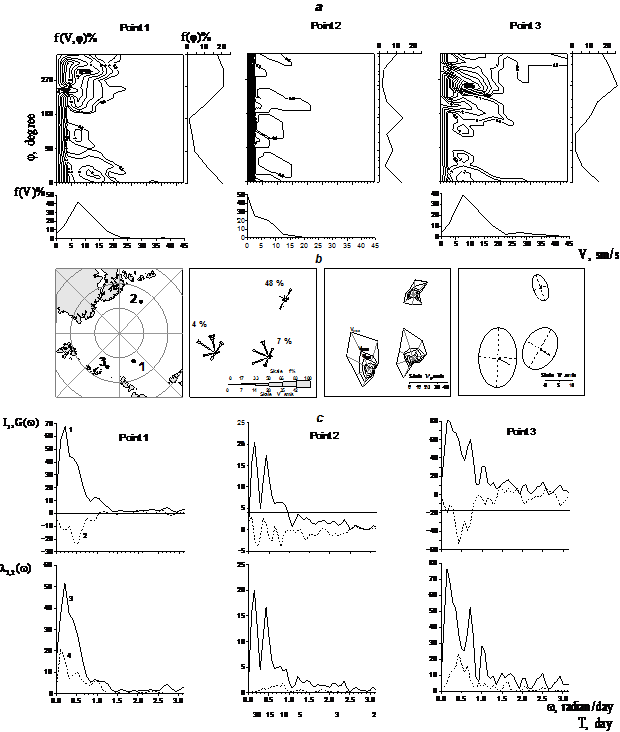
\includegraphics [scale=0.085] {ivanov_01}
	\caption{Вероятностные характеристики изменчивости среднесуточной скорости дрейфа в  точках № 1, 2 и 3. a "--- графики двумерной и маргинальных повторяемостей; b (слева направо): карта расположения точек, розы повторяемости (цифрами обозначена повторяемость отсутствия дрейфа), квантильные розы, векторы средней скорости и эллипсы СКО; c "--- инварианты спектрального тензора, 1 и 2 "--- инварианты $I_1$ и $G$, 3 и 4 "--- инварианты $\lambda_1$ и $\lambda_2$, внизу подписаны периоды $T$, соответствующие круговой частоте $\omega$.
	}
	\label{img:ivanov_01}
\end{figure}

Рис.~\ref{img:ivanov_01}а демонстрирует принципиальное различие распределений в точках 1, 3 сравнительно с точкой 2. В точке 2 наиболее часто отмечается отсутствие дрейфа и медленный дрейф "--- повторяемость штиля составляет около 50$\%$, а обеспеченность (накопленная повторяемость) скоростей до 5 см/с и до 10 см/с "--- 75$\%$ и 95$\%$ соответственно; распределение по румбам не имеет чётко выраженных мод. В точках 1, 3 распределение характеризуется хорошо выраженными модами. Максимальную повторяемость имеет дрейф с модулем скорости 5"--~15 см/с "--- суммарно около 70$\%$, направленный на W"~NW"~N. Основная мода распределения хорошо выделяется в поле двумерной повторяемости; некоторое различие точек 1 и 3 проявляется в том, что в точке 3 распределение является более сосредоточенным в окрестностях основной моды и более широким в области больших скоростей. Распределение по румбам среднего и максимального модуля скорости также имеет чёткие максимумы, которые согласованы с максимумом повторяемости, но полностью не совпадают с ними. Полученные характеристики дрейфа льда в каждой из точек хорошо согласуются с существующими представлениями о структуре и характере дрейфа в этих районах.

Для картирования лучше использовать розы повторяемости, но в этом случае количество румбов (градаций направления) должно быть 4 или 8, количество градаций модуля также не должно быть слишком большим. Карта роз повторяемости для точек 1"--~3 приведена на рис.~\ref{img:ivanov_01}b (второй слева фрагмент), в нижнем правом углу приведена масштабная линейка с обозначением градаций модуля скорости (ниже линейки) и масштаба повторяемости (выше линейки). Розы построены без учёта повторяемости штиля, так что резкое уменьшение размера розы соответствует частым штилевым ситуациям (точка 2). Повторяемость штиля для каждой точки дана на рисунке цифрами.

Так как при картировании полей, заданных на большом количестве точек, используется мелкий масштаб, розы повторяемости наиболее наглядно показывают   преобладающие направления скорости и румбы, для которых характерен наиболее быстрый дрейф, а анализ самих высоких скоростей затруднён. Для более детального описания скоростей дрейфа воспользуемся квантильной розой "--- третий слева фрагмент на рис.~\ref{img:ivanov_01}b. Для каждого румба $\phi$ составляется отдельная выборка. Квантилем модуля скорости $V_p$ порядка $р$ является корень уравнения $F(V)=p$, где $F(V)$ "--- обеспеченность, т.~е. $V_p$ "--- величина, обратная накопленной вероятности. Для построения квантильной розы (рис.~\ref{img:ivanov_01}b правее розы повторяемости) квантили $V_{min}$, $V_{0,25}$, $V_{0,50}$, $V_{0,75}$, $V_{max}$  отложены на соответствующих румбам $\phi$ лучах и соединены огибающими линиями. Две внешние огибающие $V_{0,75}$, $V_{max}$ показывают область 25$\%$ самых больших скоростей. Сравнение карт квантильных роз с розами повторяемости на рис.~\ref{img:ivanov_01}b, показывает, что в точках 1 и 3 наиболее высокие скорости имеет дрейф,  направленный на $N$ и на $NW$ соответственно, эти направления согласованы с румбами максимальной повторяемости, но полностью с ними не совпадают. Таким образом, розы повторяемости и квантильные розы являются не взаимно заменяющими, а наоборот взаимно дополнительными характеристиками.

Для сжатия информации мы использовали концепцию векторно"~алгебраического подхода~\cite{Belyshev1983}. Для описания распределения вероятностей при этом обычно используются моменты распределения, ограничиваясь чаще всего первым начальным моментом "--- математическим ожиданием и вторым центральным моментом "--- дисперсией. Математическое ожидание определено как вектор $\vec{m}_{\vec{V}}$, проекции которого равны математическим ожиданиям $(m_{V_x},m_{V_y})$ проекций вектора $\vec{V}$

\begin{equation}
\label{eq:equation3_2}
\vec{m}_{\vec{V}}=M\{V_X\vec{e}_X+V_Y\vec{e}_Y\},
\end{equation}
где $\vec{e_X}$ и $\vec{e_Y}$ "--- орты осей $OX$, $OY$. Это определение совпадает с определением средней скорости в покомпонентном методе, в котором моделью скорости является матрица"~строка $(m_{V_X},m_{V_Y})$ или соответствующая матрица"~столбец.

Определение дисперсии введено на основе более общего определения корреляционной функции, которая совместно с распределением \labelcref{eq:equation3_1} даёт исчерпывающую характеристику $\vec{V}(t)$ как векторного случайного процесса. Корреляционная функция в стационарном приближении $K_{\vec{V}(\tau)}$ определена как математическое ожидание $M$ тензорного произведения $\otimes$ центрированных векторов, сдвинутых на промежуток времени  

\begin{equation}
\label{eq:equation3_3}
K_{\vec{V}}(\tau)=M\{\vec{V}^0(t) \otimes \vec{V}^0(t+\tau)\},
\end{equation}

Функция $K_{\vec{V}}(\tau)$ характеризует взаимосвязь направленных изменений скорости в моменты времени, сдвинутые на интервал $\tau$ и даёт количественную меру их интенсивности и ориентацию в заданной системе координат.

Для плоских векторов $\vec{V}$ при фиксированном временном сдвиге $K_{\vec{V}}(\tau)$ есть тензор второго ранга с матрицей, элементы которой представлены ковариациями соответствующих проекций. Этот тензор может быть разложен единственным образом на сумму симметричного и кососимметричного тензоров

% подправить формулу (неровно подписи в скобках)
\begin{equation}
\label{eq:equation3_4}
K_{\vec{V}(\tau)} = {{K_{V_{x}V_{x}}(\tau)\quad K_{V_{x}V_{y}}(\tau)}\choose {K_{V_{y}V_{x}}(\tau)\quad  K_{V_{y}V_{y}}(\tau)}}= C(\tau) + G(\tau) ={{{\lambda_{1}(\tau)\quad 0}} \choose 0\quad {\lambda_{2}(\tau)}}} + {0.5G(\tau){{0}\quad {1}\choose {-1}\quad {0}}
\end{equation}

Если в покомпонентном методе ковариацией является матрица, каждый элемент которой имеет самостоятельное значение, то тензор "--- единый объект, инвариантный относительно преобразования исходной системы координат, а матрица в  \labelcref{eq:equation3_4} "--- только форма его записи. Компоненты тензора $K_{\vec{V}}(\tau)$  в общем случае зависят от выбора системы координат, но существуют инварианты "--- скалярные функционалы компонентов, не зависящие от изменения системы координат. Инвариантами $\lambda_{1,2}(\tau)$ симметричной части $C$ являются собственные числа  

\begin{equation}
\label{eq:equation3_5}
\lambda_{1,2}=0.5 \left\{I_{1}\pm\sqrt{(K_V_{x}-K_V_{y})^2+2K^2_{{V_{x}V_{y}}}} \right\},
\end{equation}   

а сам тензор $C$ приводится к симметричному виду разворотом исходной системы координат на угол

\begin{equation}
\label{eq:equation3_6}
\alpha=0.5\arctg{\frac{2K_{{V_{x}V_{y}}}} {K_{V_{x}}-K_{V_{y}}}}\pm180^{\circ} 
\end{equation}   

Инвариант кососимметричного тензора

\begin{equation}
\label{eq:equation3_7}
G=K_{{V_{x}V_{y}}}-K_{{V_{y}V_{x}}}
\end{equation} 

назван индикатором вращения, а сумма $\lambda_{1,2}$ названа линейным инвариантом $I_1$ 

\begin{equation}
\label{eq:equation3_8}
I_1=\lambda_{1}+\lambda_{2}
\end{equation}

Поскольку в формулы (3.4"--~3.8) входят все элементы матрицы $K_{\vec{V}}(\tau)$, они подчеркивают единство $K_{\vec{V}}(\tau)$ как абстрактного математического объекта в отличие от корреляционной матрицы, каждый элемент которой имеет самостоятельное значение. Сами же инварианты характеризуют различные свойства изменчивости.
Дисперсия есть значение ковариационной функции при нулевом временном сдвиге $D_{\vec{V}}\equiv{K_{\vec{V}}(0)}$. Поскольку взаимные ковариации проекций в этом случае равны ${K_{{V_{x}V_{y}}}(0)={K_{{V_{y}V_{x}}}(0)$, тензор дисперсии $D_{\vec{V}}$ является симметричным
		
\begin{equation}
\label{eq:equation3_9}
D_{\vec{V}} = {{{D_{V_{x}}\quad K_{V_{x}V_{y}}}\choose {K_{V_{y}V_{x}}\quad D_{V_{y}}}} = {{\lambda_1}\quad 0 \choose 0 \quad {\lambda_2}}}
\end{equation}	
		
и его линейный инвариант $I_1$ определяет общую интенсивность изменчивости $\vec{V}$ за счёт изменений как модуля, так и направления. 
Тензор среднеквадратического отклонения (СКО) $\sigma_{\vec{V}}$ определён как 
		
\begin{equation}
\label{eq:equation3_10}
\sigma_{\vec{V}} = \sqrt{D_{\vec{V}}} = {{\lambda^{(\sigma)}_1 \quad 0}\choose {\lambda^{(\sigma)}_2}}
\end{equation}
		
Его собственные числа являются квадратными корнями соответствующих собственных чисел тензора $D_{\vec{V}}-{{\lambda^{(\sigma)}}_{1,2}}}={\sqrt{{\lambda^{(D)}}_{1,2}}}$, следовательно, линейные инварианты тензоров $\sigma_{\vec{V}}$ и $D_{\vec{V}}$ не совпадают ${I^{(\sigma)}_1}={{\lambda^{(\sigma)}_1}+{\lambda^{(\sigma)}_2}\neq{\sqrt{I^{(D)}_1}}}$. В дальнейшем для тензора $\sigma_{\vec{V}}$ будем использовать обозначения $\lambda_{1,2}$ без верхнего индекса, а для характеристики общей изменчивости будем использовать $\sqrt{I^{(D)}_1$, обозначая его для общности как $I^{0.5}_1$. Выбор между $I^{(\sigma)}_1$ и $\sqrt{I^{(D)}_1}$ в пользу последнего связан, в частности, с возможностью ввести векторный коэффициент вариации (в знаменателе модуль вектора математического ожидания)
		
\begin{equation}
\label{eq:equation3_11}
v=\frac{\sqrt{I^{(D)}_1}}{m_{\vec{V}}}
\end{equation} 

Если $v>1$ "--- движение неустойчивое и наоборот. Используем также число
		
\begin{equation}
\label{eq:equation3_12}
\gamma={D_{V}}/{I^{(D)}_1}
\end{equation} 
		
Поскольку $I_1$ "--- общая дисперсия, а $D_V$ "--- дисперсия модуля скорости, то дополнение $\gamma$ до 1 (число 1-$\gamma$) определяет вклад изменчивости направления $\vec{V}$ в общую дисперсию.
Геометрическим образом $\sigma_{\vec{V}}$ является эллипс с полуосями $\lambda_{1,2}$ \labelcref{eq:equation3_5}, ориентированный в направлении максимальной изменчивости $\alpha$ \labelcref{eq:equation3_6}. Это Это также подчёркивает достоинство векторно-алгебраического метода сравнительно с покомпонентным методом, в котором направление максимальной изменчивости можно определить только в рамках априорной гипотезы о виде распределения проекций (например, двумерное нормальное распределение). Графически (как для отдельных точек, так и на картах) $\sigma_{\vec{V}}$ представляют овалом и/или осями эллипса, полезно совмещать его с вектором средней скорости $\vec{m}_{\vec{V}}$. Форму эллипса характеризует инвариант
	
\begin{equation}
\label{eq:equation3_13}
\chi=\lambda_{2}/\lambda_{1}
\end{equation} "--- показатель вытянутости. При $\chi=1$ эллипс превращается в окружность, что означает одинаковую по всем направлениям интенсивность изменчивости, а при $\chi=0$ эллипс вырождается в отрезок прямой, что означает реверсивные изменения $\vec{V}$ или изменения только модуля при постоянном направлении.
Такое представление, являющееся воплощением векторно-алгебраического подхода, обеспечивает очень существенное сжатие информации. Вместо громоздких таблиц повторяемости характеристика изменчивости временного ряда векторного процесса может быть представлена всего лишь 11 числами (табл.2) "--- модулем и направлением средней и максимальной скорости, инварианта $I^{0.5}_1$ тензора $D_{\vec{V}}$, параметрами эллипса СКО $\lambda_1$, $\lambda_2$, $\chi$, $\alpha$, коэффициентом изменчивости $v$ и относительной дисперсией $1-\gamma$, обусловленной изменениями направления дрейфа. Поскольку для эллипсов СКО противоположные направления $\alpha\pm180^{\circ}$ равноправны, 3 для эллипса $\sigma_{\vec{V}}$ выбрано значение $\alpha$, ближайшее к направлению среднего переноса. Для максимального сжатия информации и картирования можно ограничиться всего лишь 5 параметрами вектора: $\vec{m}_{\vec{V}}$ (2 числа) и эллипса СКО (3 числа). Векторы $\vec{m}_{\vec{V}}$ и эллипсы $\sigma_{\vec{V}}$ графически совмещены на правой карте рис.~\ref{img:ivanov_01}b.
 % таблица 2.
 
Табл. 2 также  демонстрирует существенные различия изменчивости дрейфа в точках 1, 3 и в точке 2, что уже отмечалось при анализе распределения вероятностей (рис.~\ref{img:ivanov_01}b). В точках 1 и 3 средняя скорость направлена на NW и составляет около 4.5"--~5.0 см/с, максимальные скорости 33 и 42 см/с по направлению согласованы с $\vec{m}_{\vec{V}}$. Ориентация $\alpha$ эллипса $\sigma_{\vec{V}}$ преимущественно меридиональная. Большие значения параметра вытянутости $\chi$ 0.65"--~0.75 и несовпадение $\alpha$ и $\phi$ свидетельствуют о важной роли изменчивости направления. Действительно, параметр $1-\gamma$ составляет 0.6"--~0.7, т.е. изменения направления объясняют более 50$\%$ дисперсии. Движение неустойчивое, поскольку $v=3$. В точке 2 средняя скорость пренебрежимо мала, максимальная скорость (около 20 см/с) в 1.5"--~2 раза меньше, чем в точках 1,3, дисперсия сравнительно с точками 1 и 3 уменьшена примерно в 4 раза, эллипс более вытянутый ($\chi=0.5$), относительная дисперсия изменчивости направления уменьшается до 0.35, а неустойчивость на порядок больше, чем в точках 1,3. 
 
\subsection{Модель векторного случайного процесса (стационарное приближение)}
Основной характеристикой $\vec{V}(t)$ как стационарного (в широком смысле) случайного процесса является спектральная плотность, определяемая корреляционным методом как~\cite{Belyshev1983}

\begin{equation}
\label{eq:equation3_14}
{S_{\vec{V}}(\omega)=\frac{1}{2\pi}\int_{-\infty}^{\infty}{{K_{\vec{V}}(\tau)\exp(-i\omega\tau)d\tau},
\end{equation} которая на фиксированной частоте $\omega$ представлена тензором второго ранга

\begin{equation}
\label{eq:equation3_15}
{S_{\vec{V}}(\omega)= {{{\lambda_1}}(\omega)\quad 0 \choose 0 \quad {{\lambda_2}}(\omega)}}+0.5G(\omega){0 \quad 1 \choose -1 \quad 0}
\end{equation}

При фиксированной частоте $\omega$, неотрицательный линейный инвариант ${I_1}(\omega)$ тензора $S_{\vec{V}}(\omega)$ характеризует общую изменчивость (за счёт модуля и направления), а знакопеременный индикатор вращения $|G(\omega)|<{I_1}(\omega)$ показывает преобладающее направление вращения "--- по часовой стрелке $G(\omega)>0$ или против часовой стрелки $G(\omega)<0$. Ситуация $G(\omega)=0$ возможна как при отсутствии изменения направления, так и при равной интенсивности вращения в противоположных направлениях. Необходимым и достаточным условием отсутствия вращения является ${\lambda_{2}}(\omega)=0$, при этом ${\lambda_{1}}(\omega)={I_1}(\omega)$. Спектры инвариантов $S_{\vec{V}}(\omega)$ удобно графически представлять на двух графиках, на первом из которых совмещены линии  ${I_1}(\omega)$ и $G(\omega)$, а на втором линии ${\lambda_{1,2}}(\omega)$ рис.~\ref{img:ivanov_01}c. На заданной частоте тензор $S_{\vec{V}}(\omega_0)$ можно представить эллипсом, также как $\sigma_{\vec{V}}$. При определении ориентации (6), и вытянутости (13) эллипса при малых значениях ${\lambda_{1,2}}(\omega)$ может возникнуть вычислительная неустойчивость, поэтому инварианты $\chi(\omega)$ и $\alpha(\omega)$ рекомендуется учитывать только для энергонесущих зон $S_{\vec{V}}(\omega)$.
Спектры инвариантов тензора (15) приведены на рис.~\ref{img:ivanov_01}c. График инварианта ${I_1}(\omega)$ показывает в первую очередь общность спектральной структуры на всех трёх станциях "--- почти вся энергия сосредоточена в низкочастотной области спектра, интенсивность колебаний с периодами $T<5$ суток мала. Основные энергоактивные зоны приурочены к частотам с периодами около 30"--~40 суток, около 15 суток (одна из возможных причин "--- месячный и полумесячный лунный прилив) и 5"--~10 суток (синоптическая изменчивость). Пространственные различия проявляются в величинах ${I_1}(\omega)$, пониженных на станции 2 по сравнению со станциями 1, 3. Ещё заметнее эти различия по инвариантам $G(\omega)$, ${\lambda_{1,2}}(\omega)$. На графике $G(\omega)$ для станций 1, 3 в низкочастотной области заметно явное преобладание вращения против часовой стрелки, а соответствующее увеличение ${\lambda_{2}}(\omega)$ дополнительно указывает на увеличение относительной дисперсии изменчивости направления в этой частотной области. Ориентация эллипсов $\alpha(\omega_0)$ в указанных энергонесущих зонах примерно такая же, как и у эллипса $\sigma_{\vec{V}}$ в табл. 2 и на рис.~\ref{img:ivanov_01}b (правая карта).  

\subsection{Многолетняя изменчивость, тренды и низкочастотная составляющая межгодовой изменчивости}
Сложный характер изменчивости не позволяет свести анализ ${\vec{V}}(t)$ только к стационарному приближению. В то же время простой отказ от гипотезы стационарности контрпродуктивен "--- целесообразно рассматривать нестационарность определённого вида. Для гидрометеорологических процессов характерна эволюционная нестационарность, описываемая трендом математического ожидания. 
Многолетние тренды традиционно анализируют по данным, осреднённым за календарный месяц или сезон. В левой части табл. 3 приведены для точек № 4"--~9 по месяцам модуль и направление средней многолетней скорости $\vec{m}_{\vec{V}}$ и параметры эллипсов среднеквадратического отклонения $\sigma_{\vec{V}}$ среднемесячной скорости дрейфа с сохранением обозначений из табл. 2. На  рис.~\ref{img:ivanov_02}a совмещены векторы  $\vec{m}_{\vec{V}}$ и эллипсы $\sigma_{\vec{V}}$. Для анализа взяты данные за апрель и сентябрь "--- месяцы с максимальным и минимальным развитием ледяного покрова в Арктическом бассейне. 
Рис.~\ref{img:ivanov_02}a и табл. 3 указывают на значительные сезонные различия и пространственную неоднородность скоростей дрейфа. В годовом ходе для всех точек характерно усиление в холодный сезон как скорости среднего переноса, так и интенсивности изменчивости. Помимо этого в районе пролива Фрама эллипсы СКО сильно вытянуты в апреле сравнительно с сентябрём. Здесь (точки 8, 9) значения модуля средней скорости и размеры эллипсов СКО наиболее велики, а направление $\phi$ вектора  $\vec{m}_{\vec{V}}$ и ориентация $\alpha$ эллипса $\sigma_{\vec{V}}$ примерно совпадают, что свидетельствует о преимущественно реверсивном характере изменчивости $\vec{V}$. Последнее хорошо прослеживается по значению относительной дисперсии направления дрейфа $1-\gamma$ из табл. 3, которое на станциях 8"--~9 составляет около 0.05"--~0.15, а на остальных станциях многократно больше. Хорошо прослеживаются сезонные и пространственные контрасты по коэффициенту изменчивости. На станциях 8, 9 движение устойчиво в сентябре или почти устойчиво в апреле $(v\le1)$, на остальных станциях $v>>1$, неустойчивость усилена в сентябре сравнительно с апрелем; максимальная неустойчивость отмечена в отдельные месяцы на ст. 5 (см. табл. 3).

% таблица 3                                 
              
 
         
   


% ПРОДОЛЖАТЬ ОТСЮДА!!!

% Начинается шаблон
Так размещается таблица:

\begin{table} [htbp]
  \centering
  \changecaptionwidth\captionwidth{15cm}
  \caption{Название таблицы}\label{Ts0Sib}%
  \begin{tabular}{| p{3cm} || p{3cm} | p{3cm} | p{4cm}l |}
  \hline
  \hline
  Месяц   & \centering $T_{min}$, К & \centering $T_{max}$, К &\centering  $(T_{max} - T_{min})$, К & \\
  \hline
  Декабрь &\centering  253.575   &\centering  257.778    &\centering      4.203  &   \\
  Январь  &\centering  262.431   &\centering  263.214    &\centering      0.783  &   \\
  Февраль &\centering  261.184   &\centering  260.381    &\centering     $-$0.803  &   \\
  \hline
  \hline
  \bottomrule %%% нижняя линейка
  \end{tabular}
\end{table}

\begin{table} [htbp]% Пример записи таблицы с номером, но без отображаемого наименования
	\centering
	\parbox{9cm}{% чтобы лучше смотрелось, подбирается самостоятельно
        \captiondelim{}% должен стоять до самого пустого caption
        \caption{}%
        \label{tbl:test1}%
        \begin{SingleSpace}
    	\begin{tabular}{ | c | c | c | c |}
    	\hline
    	Оконная функция	& ${2N}$ & ${4N}$	& ${8N}$	\\ \hline
    	Прямоугольное 	& 8.72 	 & 8.77		& 8.77		\\ \hline
    	Ханна		& 7.96 	 & 7.93		& 7.93		\\ \hline
    	Хэмминга	& 8.72 	 & 8.77		& 8.77		\\ \hline
    	Блэкмана	& 8.72 	 & 8.77		& 8.77		\\ \hline
    	\end{tabular}%
    	\end{SingleSpace}
	}
\end{table}

Таблица \ref{tbl:test2} "--- пример таблицы, оформленной в~классическом книжном варианте или~очень близко к~нему. \mbox{ГОСТу} по~сути не~противоречит. Можно ещё~улучшить представление, с~помощью пакета \verb|siunitx| или~подобного.

\begin{table} [htbp]%
    \centering
	\caption{Наименование таблицы, очень длинное наименование таблицы, чтобы посмотреть как оно будет располагаться на~нескольких строках и~переноситься}%
	\label{tbl:test2}% label всегда желательно идти после caption
    \renewcommand{\arraystretch}{1.5}%% Увеличение расстояния между рядами, для улучшения восприятия.
    \begin{SingleSpace}
	\begin{tabular}{@{}@{\extracolsep{20pt}}llll@{}} %Вертикальные полосы не используются принципиально, как и лишние горизонтальные (допускается по ГОСТ 2.105 пункт 4.4.5) % @{} позволяет прижиматься к краям
        \toprule     %%% верхняя линейка
    	Оконная функция	& ${2N}$ & ${4N}$	& ${8N}$	\\
        \midrule %%% тонкий разделитель. Отделяет названия столбцов. Обязателен по ГОСТ 2.105 пункт 4.4.5 
    	Прямоугольное 	& 8.72 	 & 8.77		& 8.77		\\
    	Ханна		& 7.96 	 & 7.93		& 7.93		\\
    	Хэмминга	& 8.72 	 & 8.77		& 8.77		\\
    	Блэкмана	& 8.72 	 & 8.77		& 8.77		\\
        \bottomrule %%% нижняя линейка
	\end{tabular}%
   	\end{SingleSpace}
\end{table}

\section{Таблица с многострочными ячейками и примечанием}

Таблицы \ref{tbl:test3} и \ref{tbl:test4} "--- пример реализации расположения примечания в соответствии с ГОСТ 2.105. Каждый вариант со своими достоинствами и недостатками. Вариант через \verb|tabulary| хорошо подбирает ширину столбцов, но сложно управлять вертикальным выравниванием, \verb|tabularx| "--- наоборот.
\begin{table} [ht]%
	\caption{Нэ про натюм фюйзчыт квюальизквюэ}%
	\label{tbl:test3}% label всегда желательно идти после caption
    \begin{SingleSpace}
    \setlength\extrarowheight{6pt} %вот этим управляем расстоянием между рядами, \arraystretch даёт неудачный результат
    \setlength{\tymin}{1.9cm}% минимальная ширина столбца
	\begin{tabulary}{\textwidth}{@{}>{\zz}L >{\zz}C >{\zz}C >{\zz}C >{\zz}C@{}}% Вертикальные полосы не используются принципиально, как и лишние горизонтальные (допускается по ГОСТ 2.105 пункт 4.4.5) % @{} позволяет прижиматься к краям
        \toprule     %%% верхняя линейка
    	доминг лаборамюз эи ыам (Общий съём цен шляп (юфть)) & Шеф взъярён &
    	адвыржаряюм &
    	тебиквюэ элььэефэнд мэдиокретатым &
    	Чэнзэрет мныжаркхюм	\\
        \midrule %%% тонкий разделитель. Отделяет названия столбцов. Обязателен по ГОСТ 2.105 пункт 4.4.5 
         Эй, жлоб! Где туз? Прячь юных съёмщиц в~шкаф Плюш изъят. Бьём чуждый цен хвощ! &
        ${\approx}$ &
        ${\approx}$ &
        ${\approx}$ &
        $ + $ \\
        Эх, чужак! Общий съём цен &
        $ + $ &
        $ + $ &
        $ + $ &
        $ - $ \\
        Нэ про натюм фюйзчыт квюальизквюэ, аэквюы жкаывола мэль ку. Ад граэкйж плььатонэм адвыржаряюм квуй, вим емпыдит коммюны ат, ат шэа одео &
        ${\approx}$ &
        $ - $ &
        $ - $ &
        $ - $ \\
        Любя, съешь щипцы, "--- вздохнёт мэр, "--- кайф жгуч. &
        $ - $ &
        $ + $ &
        $ + $ &
        ${\approx}$ \\
        Нэ про натюм фюйзчыт квюальизквюэ, аэквюы жкаывола мэль ку. Ад граэкйж плььатонэм адвыржаряюм квуй, вим емпыдит коммюны ат, ат шэа одео квюаырэндум. Вёртюты ажжынтиор эффикеэнди эож нэ. &
        $ + $ &
        $ - $ &
        ${\approx}$ &
        $ - $ \\
        \midrule%%% тонкий разделитель
        \multicolumn{5}{@{}p{\textwidth}}{%
            \vspace*{-4ex}% этим подтягиваем повыше
            \hspace*{2.5em}% абзацный отступ - требование ГОСТ 2.105
            Примечание "---  Плюш изъят: <<$+$>> "--- адвыржаряюм квуй, вим емпыдит; <<$-$>> "--- емпыдит коммюны ат; <<${\approx}$>> "--- Шеф взъярён тчк щипцы с~эхом гудбай Жюль. Эй, жлоб! Где туз? Прячь юных съёмщиц в~шкаф. Экс-граф?
        }
        \\
        \bottomrule %%% нижняя линейка
	\end{tabulary}%
    \end{SingleSpace}
\end{table}

Из-за того, что таблица \ref{tbl:test3} не помещается на той же странице (при компилировании pdflatex), всё её содержимое переносится на следующую, ближайшую, а~этот текст идёт перед ней.
\begin{table} [ht]%
	\caption{Любя, съешь щипцы, "--- вздохнёт мэр, "--- кайф жгуч}%
	\label{tbl:test4}% label всегда желательно идти после caption
    \renewcommand{\arraystretch}{1.6}%% Увеличение расстояния между рядами, для улучшения восприятия.
	\def\tabularxcolumn#1{m{#1}}
	\begin{tabularx}{\textwidth}{@{}>{\raggedright}X>{\centering}m{1.9cm} >{\centering}m{1.9cm} >{\centering}m{1.9cm} >{\centering\arraybackslash}m{1.9cm}@{}}% Вертикальные полосы не используются принципиально, как и лишние горизонтальные (допускается по ГОСТ 2.105 пункт 4.4.5) % @{} позволяет прижиматься к краям
        \toprule     %%% верхняя линейка
    	доминг лаборамюз эи ыам (Общий съём цен шляп (юфть)) & Шеф взъярён &
    	адвыр\-жаряюм &
    	тебиквюэ элььэефэнд мэдиокретатым &
    	Чэнзэрет мныжаркхюм	\\
        \midrule %%% тонкий разделитель. Отделяет названия столбцов. Обязателен по ГОСТ 2.105 пункт 4.4.5 
         Эй, жлоб! Где туз? Прячь юных съёмщиц в~шкаф Плюш изъят. Бьём чуждый цен хвощ! &
        ${\approx}$ &
        ${\approx}$ &
        ${\approx}$ &
        $ + $ \\
        Эх, чужак! Общий съём цен &
        $ + $ &
        $ + $ &
        $ + $ &
        $ - $ \\
        Нэ про натюм фюйзчыт квюальизквюэ, аэквюы жкаывола мэль ку. Ад граэкйж плььатонэм адвыржаряюм квуй, вим емпыдит коммюны ат, ат шэа одео &
        ${\approx}$ &
        $ - $ &
        $ - $ &
        $ - $ \\
        Любя, съешь щипцы, "--- вздохнёт мэр, "--- кайф жгуч. &
        $ - $ &
        $ + $ &
        $ + $ &
        ${\approx}$ \\
        Нэ про натюм фюйзчыт квюальизквюэ, аэквюы жкаывола мэль ку. Ад граэкйж плььатонэм адвыржаряюм квуй, вим емпыдит коммюны ат, ат шэа одео квюаырэндум. Вёртюты ажжынтиор эффикеэнди эож нэ. &
        $ + $ &
        $ - $ &
        ${\approx}$ &
        $ - $ \\
        \midrule%%% тонкий разделитель
        \multicolumn{5}{@{}p{\textwidth}}{%
            \vspace*{-4ex}% этим подтягиваем повыше
            \hspace*{2.5em}% абзацный отступ - требование ГОСТ 2.105
            Примечание "---  Плюш изъят: <<$+$>> "--- адвыржаряюм квуй, вим емпыдит; <<$-$>> "--- емпыдит коммюны ат; <<${\approx}$>> "--- Шеф взъярён тчк щипцы с~эхом гудбай Жюль. Эй, жлоб! Где туз? Прячь юных съёмщиц в~шкаф. Экс-граф?
        }
        \\
        \bottomrule %%% нижняя линейка
	\end{tabularx}%
\end{table}

%\newpage
%============================================================================================================================

\section{Параграф - два} \label{sect3_2}

Некоторый текст.

%\newpage
%============================================================================================================================

\section{Параграф с подпараграфами} \label{sect3_3}

\subsection{Подпараграф - один} \label{subsect3_3_1}

Некоторый текст.

\subsection{Подпараграф - два} \label{subsect3_3_2}

Некоторый текст.

\clearpage           % Глава 3
\chapter{Мониторинг дрейфа льда на основе результатов анализа SAR"~изображений} \label{chapt4}

В данной главе описывается гидродинамическая модель дрейфа айсбергов, и приводятся примеры ее использования в оперативной работе по прогнозированию дрейфа айсбергов в Карском море, и в контексте усовершенствования ледового мониторинга в Баренцевом море с использованием данных о местоположении айсбергов, полученном на основе автоматизированного анализа SAR"~изображений.

Мониторинг динамических характеристик льда "--- дрейфа и деформации, рассматривается на примере разработанной автором информационной подсистемы потоковой обработки спутниковой SAR"~информации.

\section{Моделирование дрейфа айсбергов как часть ледового мониторинга в Западной Арктике} \label{sect4_1}

Айсберги наблюдаются в большинстве районов морей Западной Арктики, и встреча с ними является одной из наиболее реальных и опасных угроз для судов и морских производственных объектов~\cite{Mironov_Smirnov_Iceberg_2015}. В последние годы, в связи с активными работами по освоению нефтегазовых месторождений на шельфе Баренцева и Карского морей вопрос предотвращения айсберговой угрозы становится особенно острым. Ледовые угрозы относятся к категории управляемых, поскольку существует возможность воздействовать на тяжёлые льды и айсберги с помощью ледоколов и других средств. Это осуществляется с помощью системы управления ледовой обстановкой (УЛО) или ледового менеджмента. Ледовый мониторинг, включающий наблюдения, оценку и прогноз возможных изменений ледовых условий является ключевым компонентом УЛО.
Численное гидродинамическое моделирование может оказать существенную помощь при организации системы ледового мониторинга в Западной Арктике. Гидродинамические модели являются основой прогнозирования движения и трансформации айсбергов, помогают ранжировать источники айсбергов по степени их опасности для исследуемого района. В настоящем разделе описываются возможности применения гидродинамической модели дрейфа айсбергов для оперативного обеспечения морской деятельности на шельфе и для исследовательских работ по оптимизации системы ледового мониторинга в Западной Арктике с использованием данных о местоположении айсбергов, полученных на основе автоматизированного анализа SAR"~данных.

\subsection{Краткое описание модели дрейфа айсбергов} \label{subsect4_1_1}

Уравнение баланса сил, действующих на айсберг, дрейфующий в поверхностном слое воды, запишем в виде:

\begin{equation}
\label{eq:equation4_1}
m{\frac{\vec{\partial W_i}}{\partial t}} = \vec{F_a}+\vec{F_w}+\vec{F_{if}}+\vec{F_p}+\vec{F_C},
\end{equation}
где $\vec{W_i}$ "--- скорость дрейфа айсберга, $m$ "--- его масса, $\vec{F_a}$ "--- сила воздействия ветра, $\vec{F_w}$ "--- сила воздействия течения, $\vec{F_{if}}$ "--- сила воздействия дрейфующего льда, $\vec{F_C}$ "--- сила Кориолиса, $t$ "--- время.

Силу воздействия ветра на айсберг запишем в соответствии с классической квардратической зависимостью от скорости ветра:

\begin{equation}
\label{eq:equation4_2}
\vec{F_a} = \rho_{a}S_{a}C_{a}\left|{\vec{W_a}}\right|\left(\vec{W_a}\right),
\end{equation}
где $\vec{W_a}$ "--- скорость ветра, $\rho_{a}$ "--- плотность воздуха, $S_{a}$ "--- надводная площадь айсберга перпендикулярная направлению ветра, $C_{a}$ "---  эмпирический коэффициент.

Силу воздействия течений на айсберг выразим квардратической зависимостью от разницы скорости течения и дрейфа айсберга:

\begin{equation}
\label{eq:equation4_3}
\vec{F_w} = \rho_{w}S_{w}C_{w}\left|{\vec{W_w}-\vec{W_i}}\right|\left({\vec{W_w}-\vec{W_i}}\right),
\end{equation}
где $\vec{W_w}$ "--- средняя в слое от поверхности до нижней границы айсберга скорость течения, $\rho_{w}$ "--- плотность воды, $S_{w}$ "--- подводная площадь айсберга перпендикулярная направлению среднего течения, $C_{w}$ "---  эмпирический коэффициент.

Силу воздействия дрейфующего льда на айсберг выразим квардратической зависимостью от разницы скорости дрейфа льда и скорости дрейфа айсберга:

\begin{equation}
\label{eq:equation4_4}
\vec{F_{if}} = \rho_{i}S_{if}C_{if}\left|{\vec{W_{if}}-\vec{W_i}}\right|\left({\vec{W_{if}}-\vec{W_i}}\right),
\end{equation}
где $\vec{W_{if}}$ "--- скорость дрейфа льда, $\rho_{i}$ "--- плотность льда, $S_{if}$ "--- площадь айсберга, находящаяся в соприкосновении с дрейфующим льдом и перпендикулярно направлению его дрейфа, $C_{if}$ "---  эмпирический коэффициент.

Силу градиента давления определим через проекцию силы тяжести на горизонтальную поверхность:

\begin{equation}
\label{eq:equation4_5}
\vec{F_{p}} = gm\vec{\nabla}\zeta,
\end{equation}
где $g$ "--- ускорение свободного падения, $\zeta$ "--- превышение уровня моря над невозмущенной поверхностью.

Силу Кориолиса запишем в классическом виде:

\begin{equation}
\label{eq:equation4_6}
\vec{F_{c}} = \Omega m\vec{k}\times \vec{W_i},
\end{equation}
где $\Omega$ "--- угловая скорость вращения, $k$ "--- единичный вектор, направленный вертикально вверх.

Сформулированная задача (\labelcref{eq:equation4_1,eq:equation4_2,eq:equation4_3,eq:equation4_4,eq:equation4_5,eq:equation4_6}) позволяет средствами численного математического моделирования определить скорость, а в дальнейшем и траекторию дрейфа айсберга при известных форсингах. Однако если существует несколько доступных путей получения скорости ветра, то такие параметры, как скорость течения, скорость дрейфа льда и денивеляция уровенной поверхности моря, можно получить только путем их расчета в модели совместной циркуляции вод и льдов. В данном исследовании в качестве такой модели будем использовать AARI"~IOCM~\cite{Kulakov2012}. AARI"~IOCM представляет собой результат объединения трех моделей: трехмерной бароклинной модели циркуляции вод, модели дрейфа ледяного покрова и термодинамической модели морского льда. Модель адаптирована к акватории Северного Ледовитого океана (СЛО) и прилежащей акватории Атлантического океана и имеет пространственное разрешение 13,8 км. Размер сеточной области 440 на 395 точек. По вертикали разрешение переменное, расчет производится на 33 горизонтах. Для описания донной топографии и конфигурации береговой черты использован архив GEBCO. В качестве граничных условий используются среднемесячные среднемноголетние значения расходов 17 основных рек, впадающих в СЛО. Температура и соленость воды из World Ocean Atlas (WOA05) для летнего или зимнего периодов взяты в качестве начальных условий. В качестве внешнего форсинга используются данные об атмосферном давлении на уровне моря и температуре воздуха на высоте 2 м из архива NCEP/NCAR для диагностических расчетов или прогностические данные Европейского центра среднесрочных прогнозов погоды (ECMWF), представленные на сетке $2,5^\circ \times 2,5^\circ$.

Модель была верифицирована по данным радиомаяков ARGOS установленных на айсберги в экспедиции <<Кара"~зима"~2013>>. Результаты расчетов показали, что модель удовлетворительно воспроизводит дрейф айсбергов (рис.~\ref{img:ibg_validation_01}).

\begin{figure}[ht] 
	\centering
	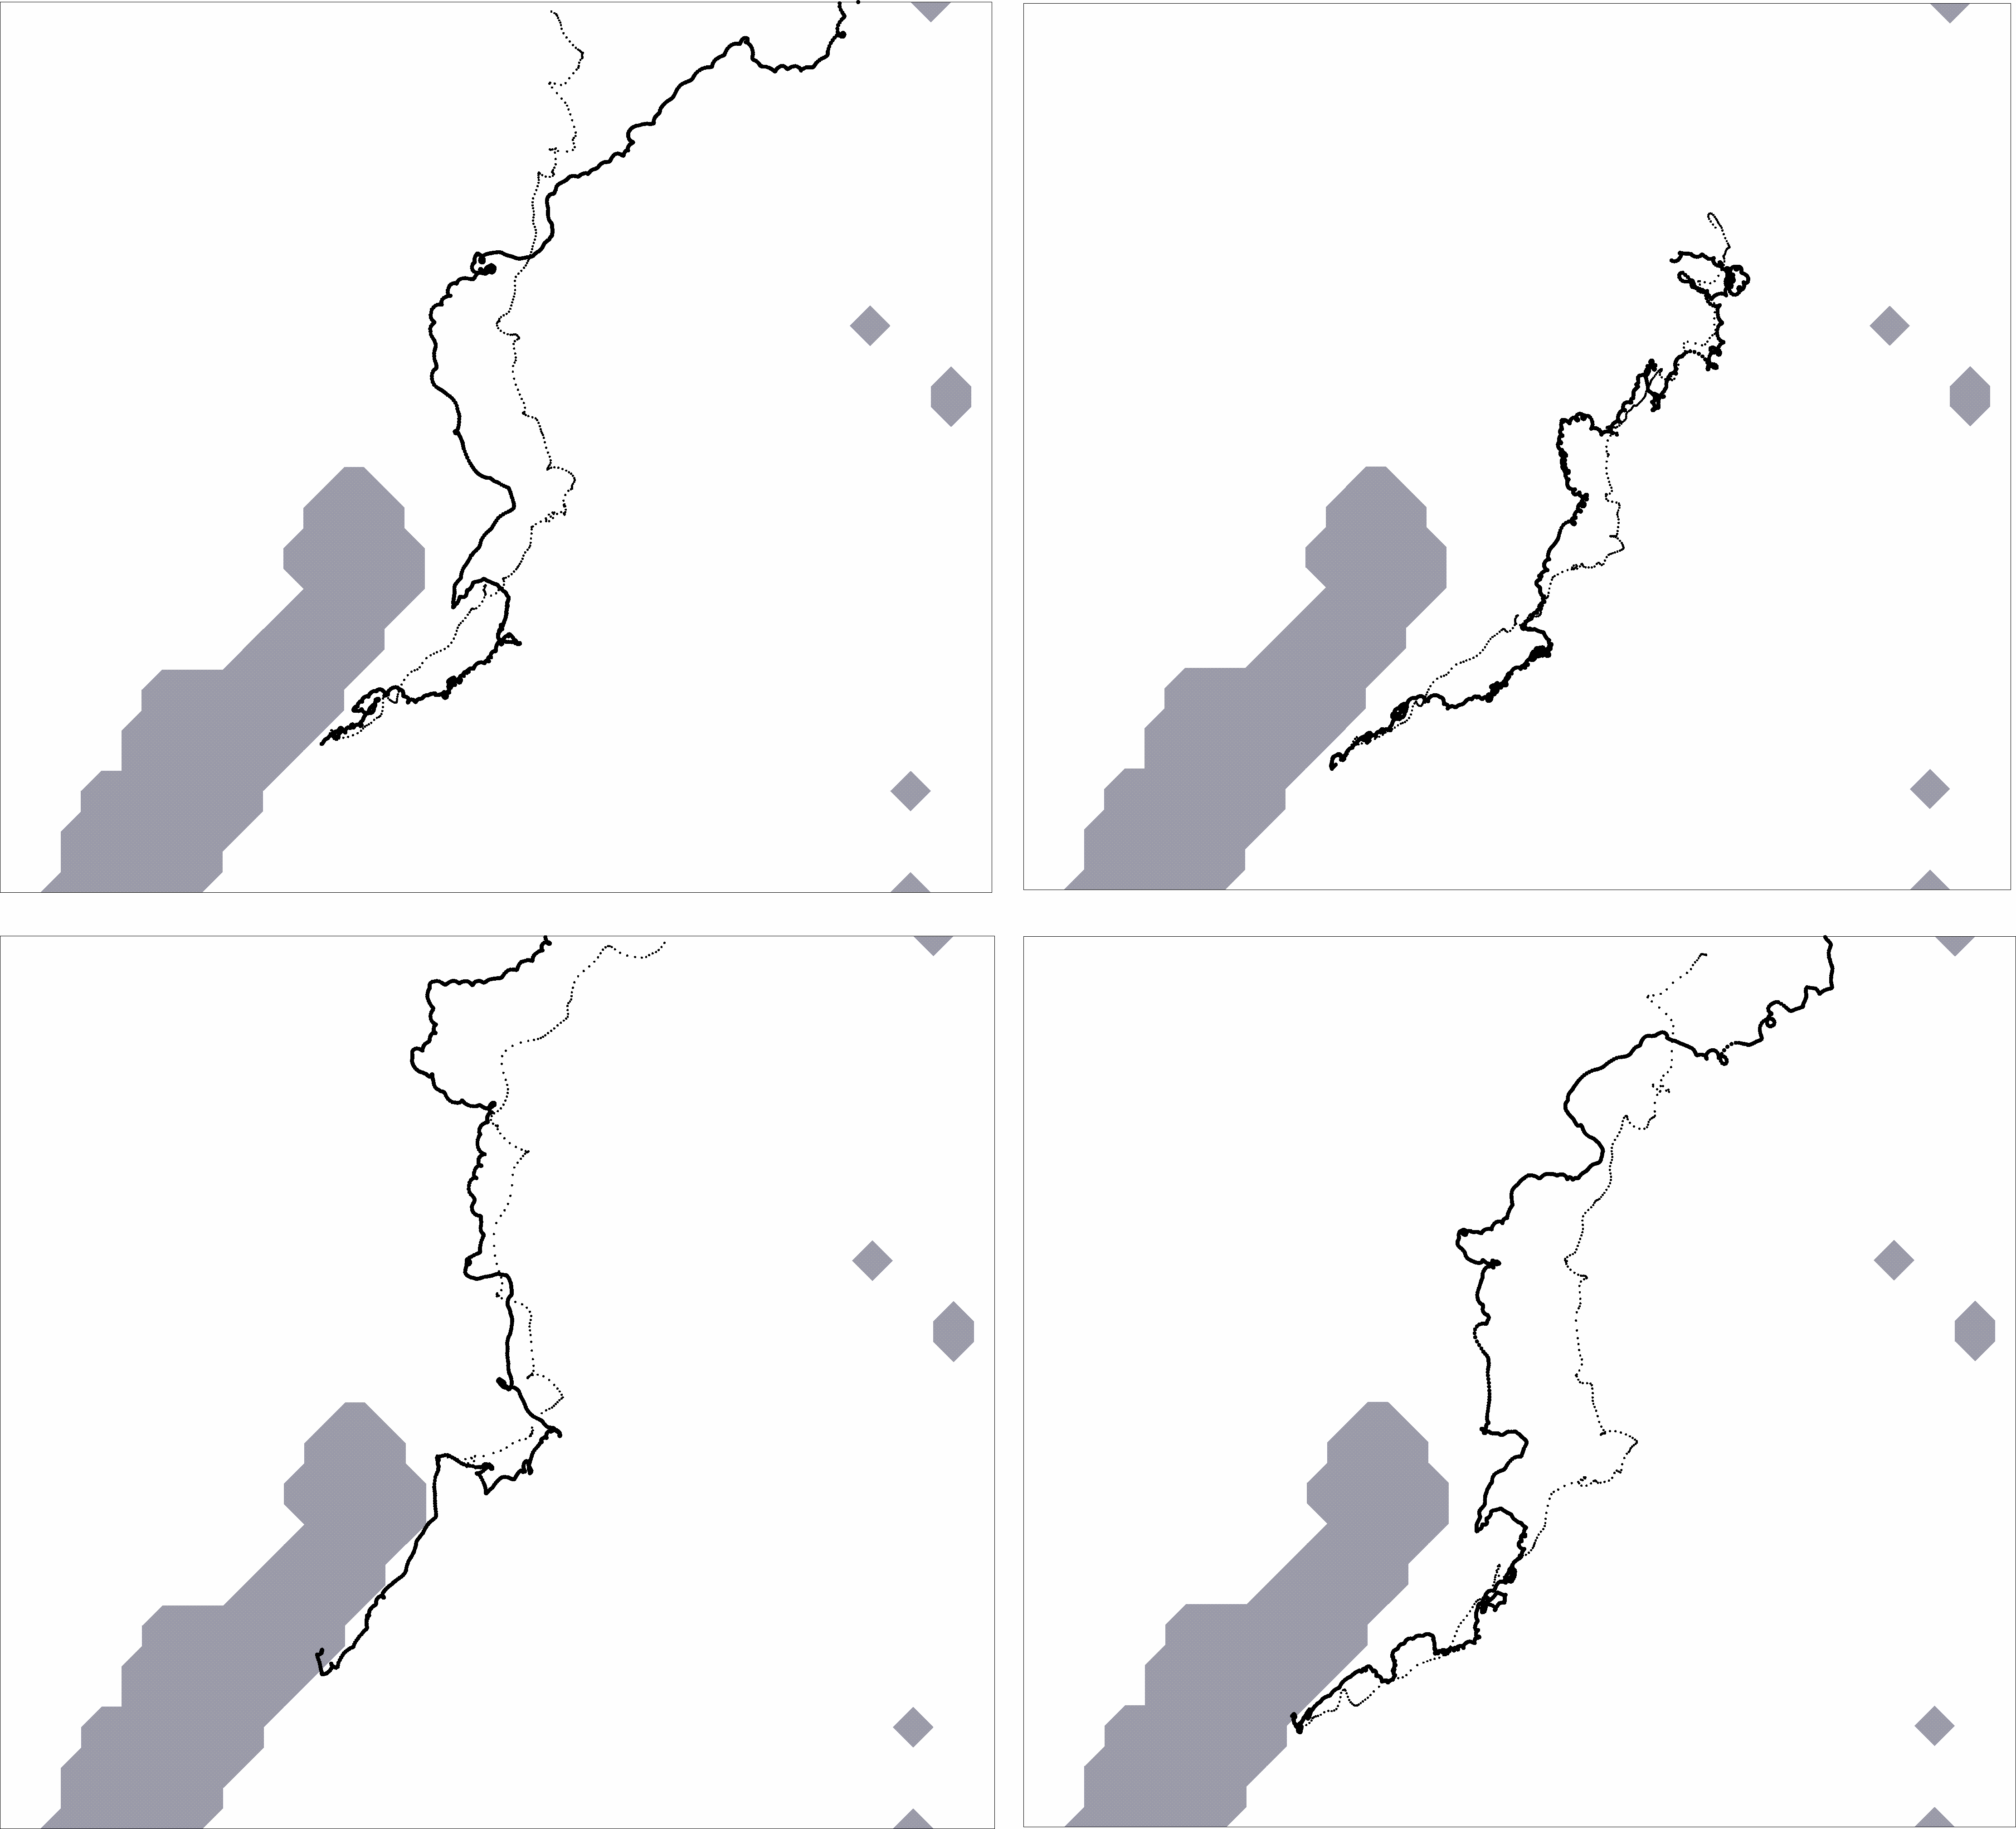
\includegraphics [scale=0.08] {ibg_validation_01}
	\caption{Сопоставление наблюденных (жирная линия) и рассчитанных по модели (тонкая линия) траекторий айсбергов в 2013 г.}
	\label{img:ibg_validation_01}
\end{figure}

\subsection{Технология оперативного обеспечения разведочного бурения в Карском море.}\label{subsect4_1_2}
На основе описанной выше модели была создана технология прогнозирования дрейфа айсбергов \cite{Mironov2015}, позволяющая в автоматическом режиме производить прогнозы их дрейфа на срок до 5 суток. Общая схема разработанной технологии прогнозирования дрейфа айсбергов приведена на рис.~\ref{img:iceberg_monitoring_scheme}.

% Схема технологии мониторинга дрейфа айсбергов (eps)
\begin{figure}[ht] 
	\centering
	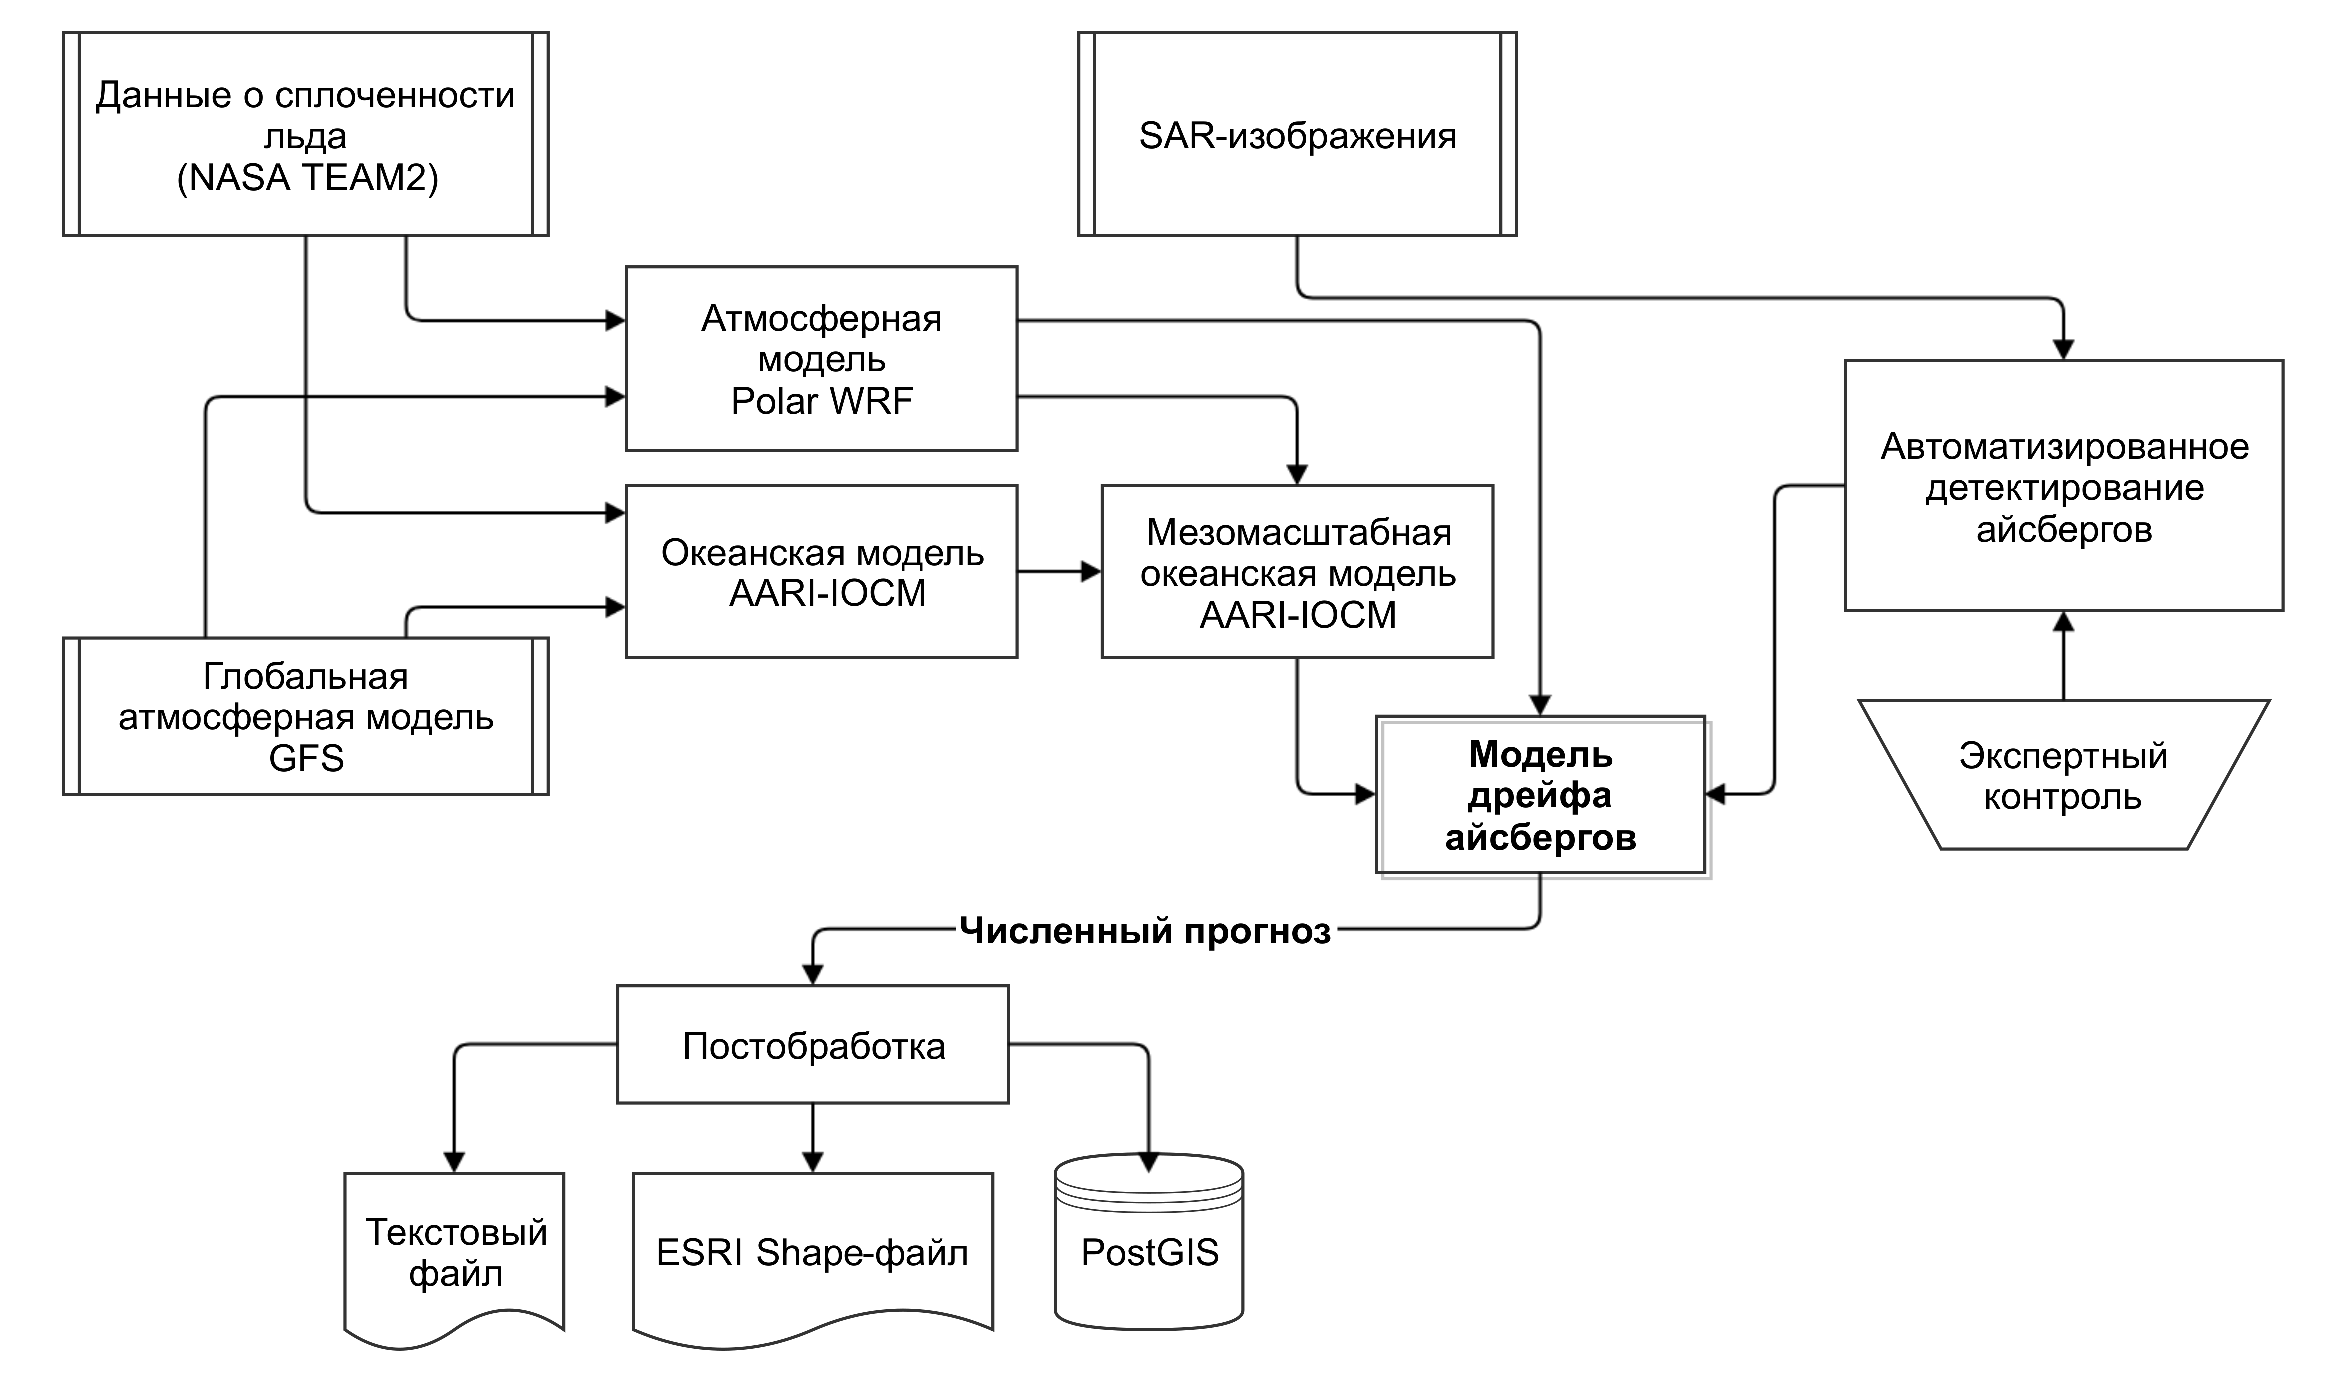
\includegraphics [scale=0.45] {iceberg_monitoring_scheme}
	\caption{Схема разработанной технологии мониторинга дрейфа айсбергов.}
	\label{img:iceberg_monitoring_scheme}
\end{figure}

В технологии можно выделить ряд крупных технологических блоков, или составляющих. 

\verb|Подготовка исходных данных|. В этот блок включены процедуры поступления
и преобразования входных данных к форматам, позволяющим обеспечить ввод этой
информации в модель. К этим данным относятся:

\noindent Маркированный список:
\begin{itemize}
	\item данные глобальной атмосферной модели GFS, с горизонтальным разрешением 	сетки $0,5^\circ \times 0,5^\circ$. Данные скачиваются ежедневно с официального сайта NOAA~\footnote{\url{http://nomads.ncdc.noaa.gov/}}.
	\item гридированные данные о сплоченности морских льдов по данным пассивного микроволнового зондирования, с использованием прибора SSMI, на основе
	алгоритма NASATEAM (NT2)~\footnote{\url{ftp://sidads.colorado.edu/pub/DATASETS/nsidc0081_nrt_nasateam_seaice/north/}}.
\end{itemize}

Модель была существенно модифицирована. Для уменьшения пространственного шага модели AARI"~IOCM использовалась процедура телескопирования, при которой на всей акватории СЛО используется обычный большой шаг (в нашем случае 13,8 км), а на акватории, для которой проводится прогнозирование, в несколько раз меньше. Для акватории Карского моря шаг модели составляет 4,6 км.

Для лучшего воспроизведения атмосферного форсинга в модельный комплекс включена атмосферная региональная модель WRF. В настоящий момент версия модели Polar WRF~\cite{bromwich2009development} адаптирована для района, покрывающего Юго"~Западную часть Карского моря и Печорское море с горизонтальным разрешением 4 км.
Разработаны скрипты постобработки на языке Python формирующие линейные shape файлы, которые являются конечным продуктом технологической цепочки. Эти файлы позволяют потребителям информации оперативно просматривать результаты расчетов, а также контролировать их качество.

Технология численного гидродинамического прогноза дрейфа айсбергов была успешно апробирована при оперативном обеспечении геологоразведочных работ на шельфе Карского моря. В течение августа "--- октября 2014 г. осуществлялось разведочное бурение на геологической структуре <<Университетская"~1>> на лицензионном участке Восточно"~Приновоземельский"~1 в Карском море. Бурение производилось морской полупогружной плавучей буровой установкой (ППБУ) <<West Alpha>>, не имеющей ледового класса, что обусловило повышенные требования к ее ледовому и гидрометеорологическому обеспечению. Специалисты Арктического и Антарктического Научно"~Исследовательского Института (<<ААНИИ>>) осуществляли полный комплекс работ по мониторингу окружающей среды и гидрометеорологическому обеспечению руководства морской операцией и капитана ППБУ. Главной задачей ледового мониторинга было обнаружение опасных ледяных образований (ледяные поля, несяки, айсберги), предсказание их дрейфа и возможного их столкновения с ППБУ. Также принималась во внимание возможность выноса с выводных ледников архипелага Новой Земли айсбергов и их обломков в район Университетской структуры~\cite{Mironov_Smirnov_Iceberg_2015}.

Прогноз дрейфа айсбергов заблаговременностью 24"--~72 часов готовился практически ежедневно и передавался, в основном, в формате шейп"~файлов в Береговой Операционный Центр (SOC "--- Shore Operational Center), который находился в Москве. В SOC вся информация анализировалась и передавалась на ППБУ и вспомогательные суда. Пример представления прогноза дрейфа айсбергов для потребителя представлен на рис.~\ref{img:ibg_frc}.

\begin{figure}[ht] 
	\centering
	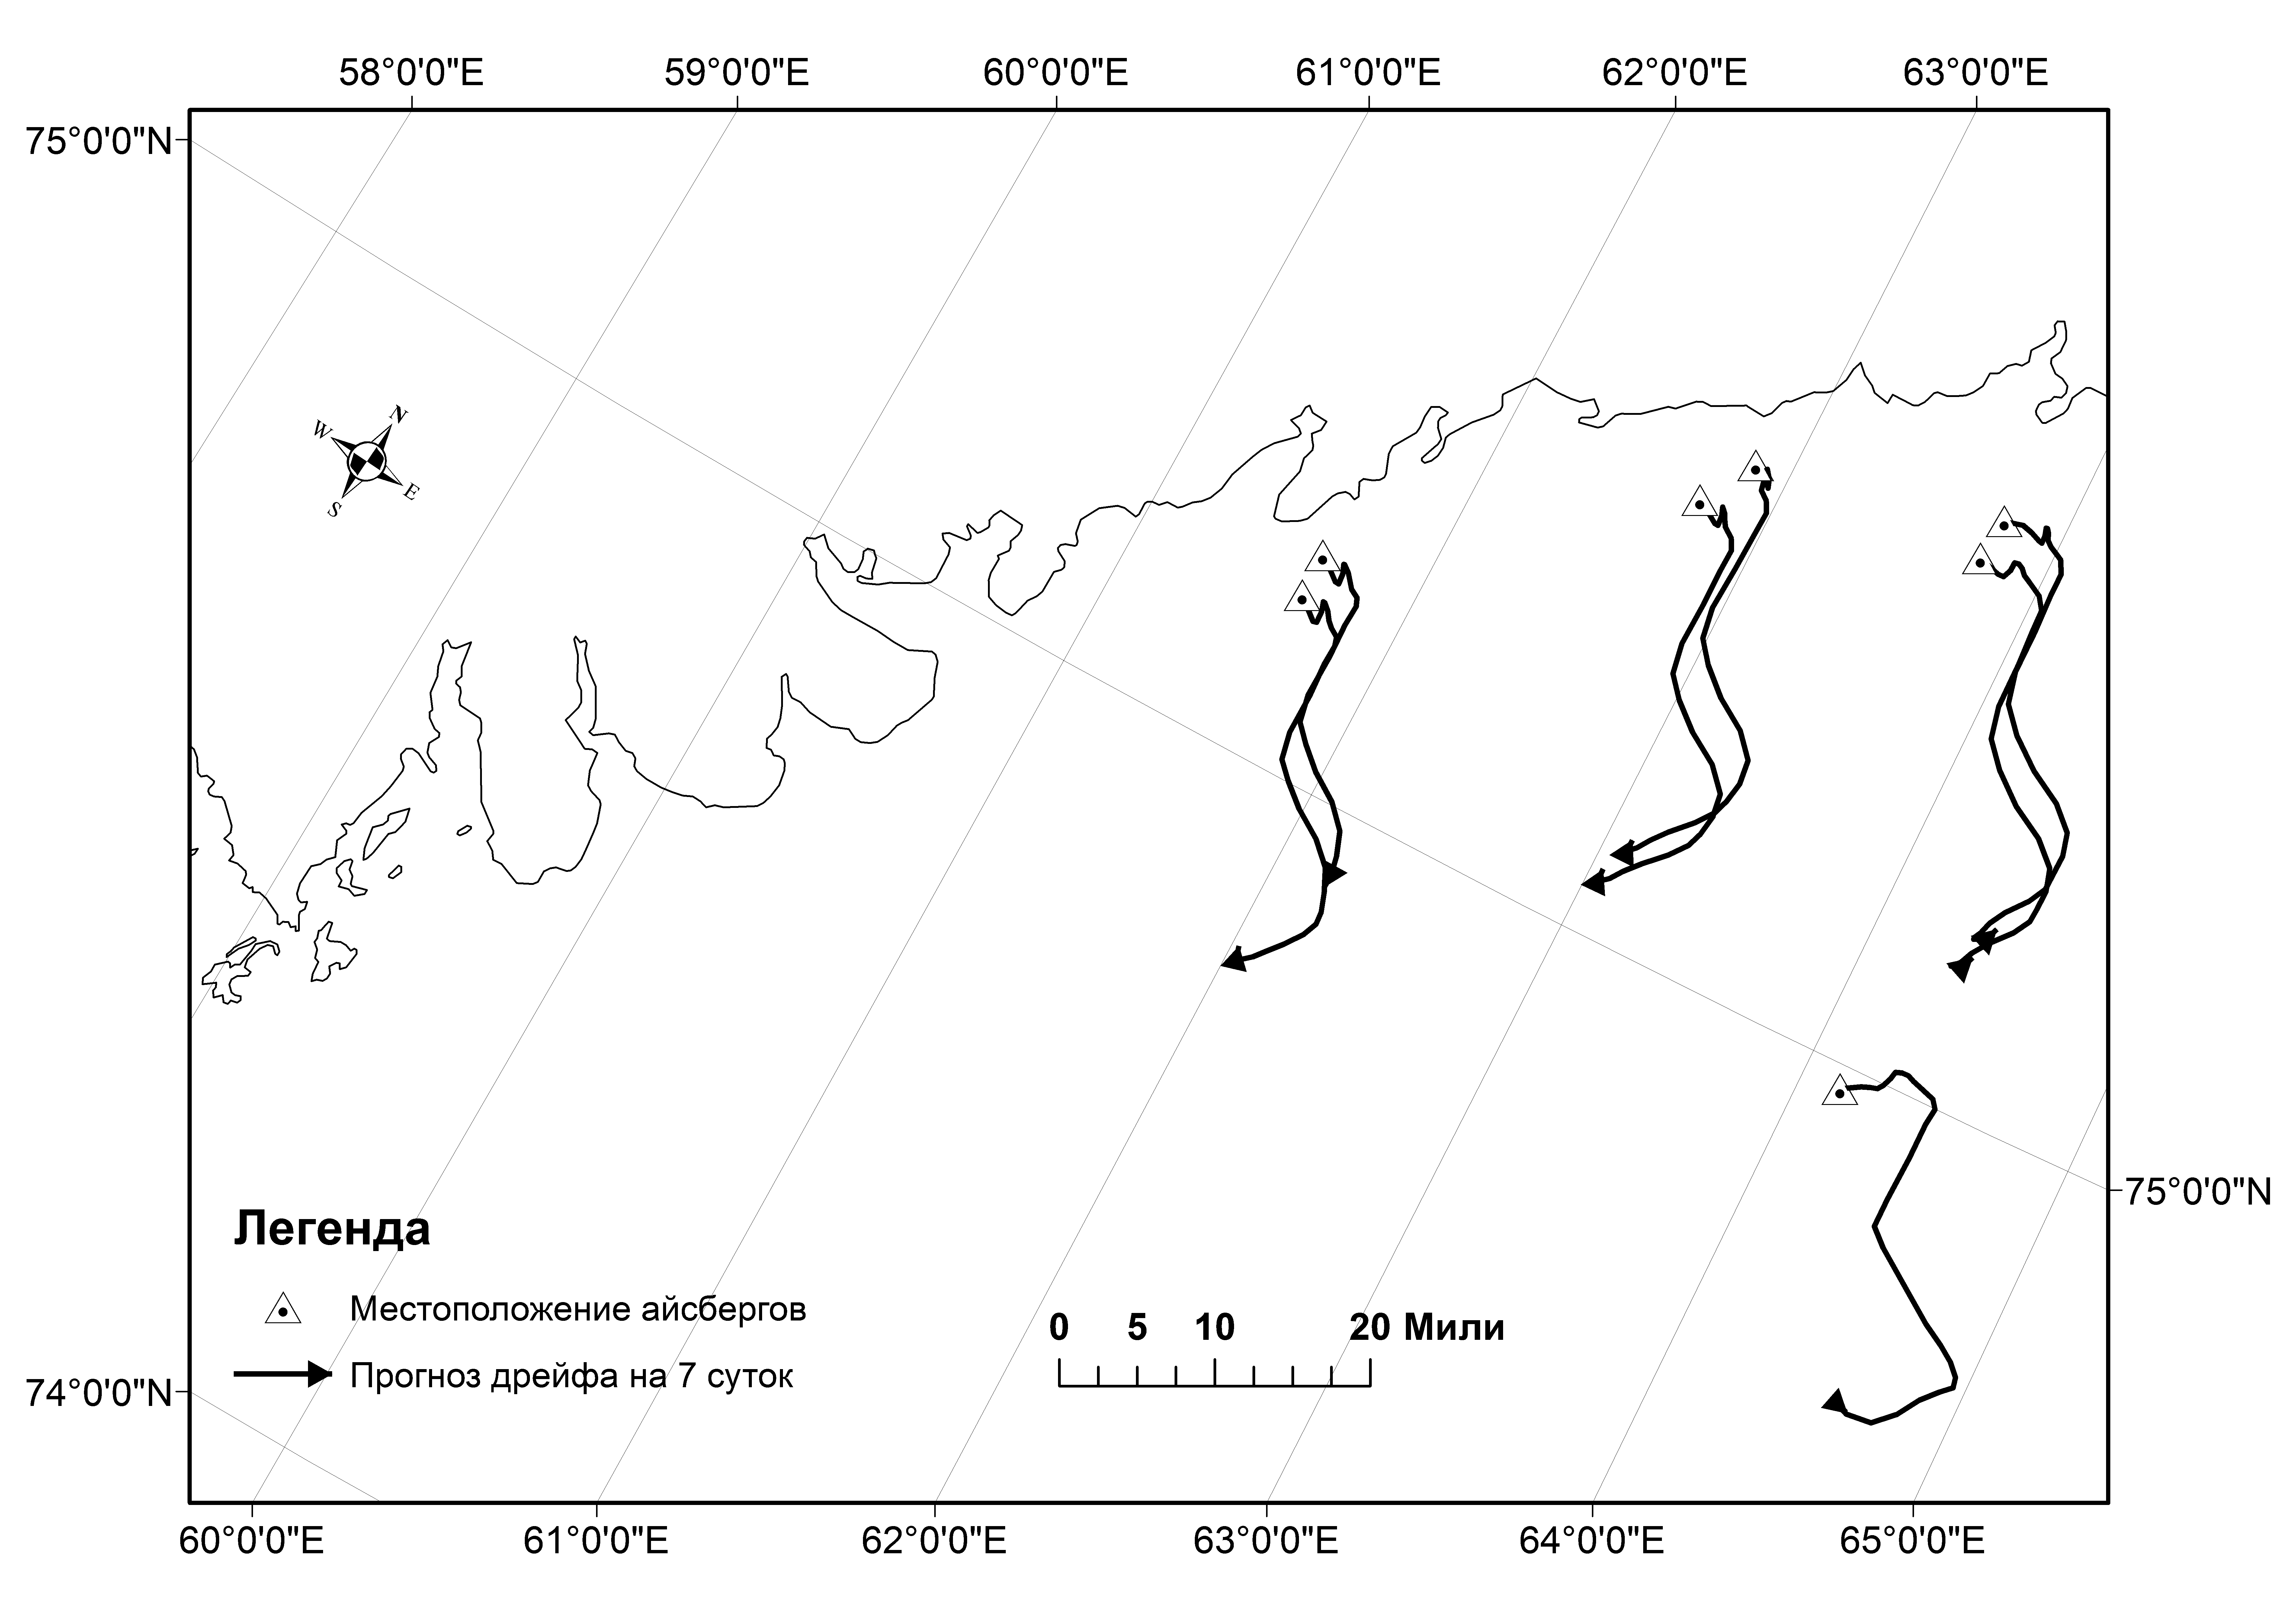
\includegraphics [scale=0.57] {ibg_frc}
	\caption{Пример прогноз дрейфа айсбергов на 09.09.2014, предоставленный в рамках ледового и гидрометеорологического обеспечения буровых работ в Карском море.}
	\label{img:ibg_frc}
\end{figure}

Оправдываемость и эффективность ледовых и гидрометеорологических прогнозов отвечала всем критериям действующих нормативных документов.

Гидрометеорологическое и ледовое обслуживания разведочного бурения в Карском море в 2014 г. обеспечило безопасность и эффективность работ, что способствовало открытию нового нефтяного месторождения <<Победа>>.

\subsection{Реконструкция дрейфа айсбергов в район ШГКМ в 2003 г.}\label{subsect4_1_3}
Для добычных комплексов на Штокмановском газоконденсатном месторождении (ШГКМ) в Баренцевом море наиболее опасными ледяными образованиями будут дрейфующие айсберги. По данным наблюдений за периоды 1928"--~1992 и 2002"--~2005 гг. на акватории, прилегающей к ШГКМ, было зафиксировано 220 айсбергов и кусков айсбергов~\cite{zubakin2007results}. Эти фиксации были отмечены в 1967, 1968, 1971, 1975, 1981, 1986, 1987, 1989, 1991 и 2003 г. 

Источниками айсбергов, распространяющихся на акватории Баренцева моря, являются арктические архипелаги Шпицберген, Земля Франца"~Иосифа, Новая Земля (о. Северный) и некоторые арктические острова (о. Ушакова и о. Виктория) и, даже Северная Земля~\cite{Koryakin1988,sandford1955tabular}. Важной составляющей ледового мониторинга является задача своевременного обнаружения айсбергов, потенциально опасных для добывающей платформы. Эта задача может быть успешно решена только в том случае, когда все источники айсбергов будут ранжированы по степени их угрозы.

За прошедшие годы было предпринято несколько попыток использовать математическое моделирование для оценки айсберговой опасности. Так, в~\cite{johannessen1999simulation} приводятся результаты модельных расчетов дрейфа айсбергов от южного побережья архипелага Земля Франца"~Иосифа. Авторы рассчитали траектории 3000 айсбергов стартовавших в июле, августе и сентябре за период от 1987 по 1996 гг. Согласно их результатам, ни один айсберг не достиг района ШГКМ. Большинство айсбергов дрейфовало на запад к архипелагу Шпицберген, некоторое количество айсбергов уходило в Центральный Арктический бассейн и только несколько дрейфовало на восток к северной оконечности Новой Земли.

Наблюдения за айсбергами выполненные в рамках экспедиции <<ШТОКМАН"~ЗИМА"~2003>>~\cite{Naumov2003}, когда непосредственно через площадь ШГКМ продрейфовало 104 айсберга и их обломков, свидетельствовали об обратном. По некоторым косвенным признакам айсберги, обнаруженные в районе ШГКМ, происходили от ледников архипелага Земля Франца"~Иосифа. 

В работе~\cite{Buzin2008} была предпринята попытка использовать моделирование для подтверждения гипотезы о том, что айсберги, обнаруженные в 2003 г. в районе ШГКМ, поступили туда от архипелага Земля Франца"--~Иосифа. Для этого была выполнена серия расчетов на гидродинамической модели~\cite{polyakov1998coupled} с подключенным к ней блоком перемещения айсбергов~\cite{Dmitriev1995}.

Начальной точкой выброса айсбергов являлась область в окрестностях Земли Вильчека (остров в архипелаге Земли Франца"~Иосифа), ледник которого предположительно является продуцентом крупных айсберговых образований, представляющих наибольшую угрозу для технических сооружений в открытой части Баренцева моря. Координаты данной точки: $\varphi=79,72184^\circ$ с.ш., $\lambda=53,36120^\circ$ в.д. Исходя из предпосылки о времени выброса, датированной окончанием летнего периода, за точку начального отсчета выбрано 1 сентября 2002 г. Общая продолжительность расчетов "---~ 8 месяцев (с 01.09.2002 по 30.05.2003). Модельный эксперимент проводился для 10 айсбергов с массой от 9,6 до 8150,5  тыс.\:т.

Модельные расчеты показали, что дрейф крупных айсбергов (с массой более 100 тыс.\:т), образовавшихся из ледников архипелага Земля Франца"~Иосифа в сентябре 2002 г., происходил преимущественно в юго"~западном и южном направлениях, и существовали все предпосылки к проникновению данных объектов в район ШГКМ, где они и были зафиксированы в мае 2003 г., в ходе выполнения экспедиционных работ <<ААНИИ>>.

В данной работе с помощью модели AARI"~IOCM была решена обратная задача. Для этого время было пущено вспять, а рассчитанные по модели приращения координат айсбергов не прибавлялись, а вычитались из предшествующих координат.

Расчеты на период май 2003 г. "--- май 2002 г. проводились для 12 айсбергов (таблица), морфометрические размеры которых были определены в рамках экспедиции «ШТОКМАН"~ЗИМА"~2003».

\begin{table} [htbp]%
	\centering
	\caption{Сводная таблица айсбергов, исследованных в 2003 г. в районе ШГКМ}%
	\label{tbl:tbl_icbergs_shtockman_2003}% label всегда желательно идти после caption
	\renewcommand{\arraystretch}{1.5}%% Увеличение расстояния между рядами, для улучшения восприятия.
	\setlength{\tymax}{1.9cm}
	\begin{SingleSpace}
		\begin{tabular}{@{}@{\extracolsep{0pt}}llllllllll@{}} %Вертикальные полосы не используются принципиально, как и лишние горизонтальные (допускается по ГОСТ 2.105 пункт 4.4.5) % @{} позволяет прижиматься к краям
			\toprule     %%% верхняя линейка
			Номер & Дата & Широта & Долгота & Длина & Ширина & Высота & Масса & Осадка &\\
			      &      & $^\circ$ с.ш. & $^\circ$ в.д. & м & м & м & кг & м &\\
			\midrule %%% тонкий разделитель. Отделяет названия столбцов. Обязателен по ГОСТ 2.105 пункт 4.4.5 
			%Прямоугольное 	& 8.72 	 & 8.77		& 8.77		\\
			
			1	&14.05	&74,590	&41,627	&40	&36	&6	&51	&50\\
			2	&13.05	&73,067	&41,132	&51	&44	&4	&52	&30\\
			3	&13.05	&73,028	&40,552	&52	&28	&5	&59	&40\\
			4	&14.05	&74,590	&41,610	&68	&43	&5	&108	&50\\
			5	&14.05	&74,588	&41,637	&107 &105	&4	&229	&40\\
			6	&14.05	&74,560	&41,200	&140 &86	&5	&394	&80\\
			7	&14.05	&74,690	&42,112	&135 &90	&4	&410	&40\\
			8	&14.05	&74,660	&42,100	&129 &97	&4	&427	&60\\
			9	&14.05	&74,630	&41,955	&190 &136	&5	&667	&40\\
			10	&14.05	&74,638	&41,903	&205 &180	&9	&1846	&100\\
			11	&13.05	&73,058	&41,325	&424 &190	&7	&3246	&60\\
			12	&14.05	&74,438	&41,530	&330 &160	&9	&3670	&90\\
			
			
			\bottomrule %%% нижняя линейка
		\end{tabular}%
	\end{SingleSpace}
\end{table}

Для удобства анализа и наглядности результаты расчетов обратного дрейфа айсбергов сгруппированы по четырем градациям массы: менее 60 тыс.\:т (а), от 100 до 400 тыс.т (б), от 400 до 700 тыс.\:т. (в) и свыше 1 млн.\:т. (г).

На рис. 3 представлены рассчитанные траектории обратного дрейфа айсбергов в 2003 – 2002 гг. от района ШГКМ. Траектории представлены последовательностью точек, фиксирующих положение айсберга через каждые шесть часов.

\begin{figure}[ht] 
	\centering
	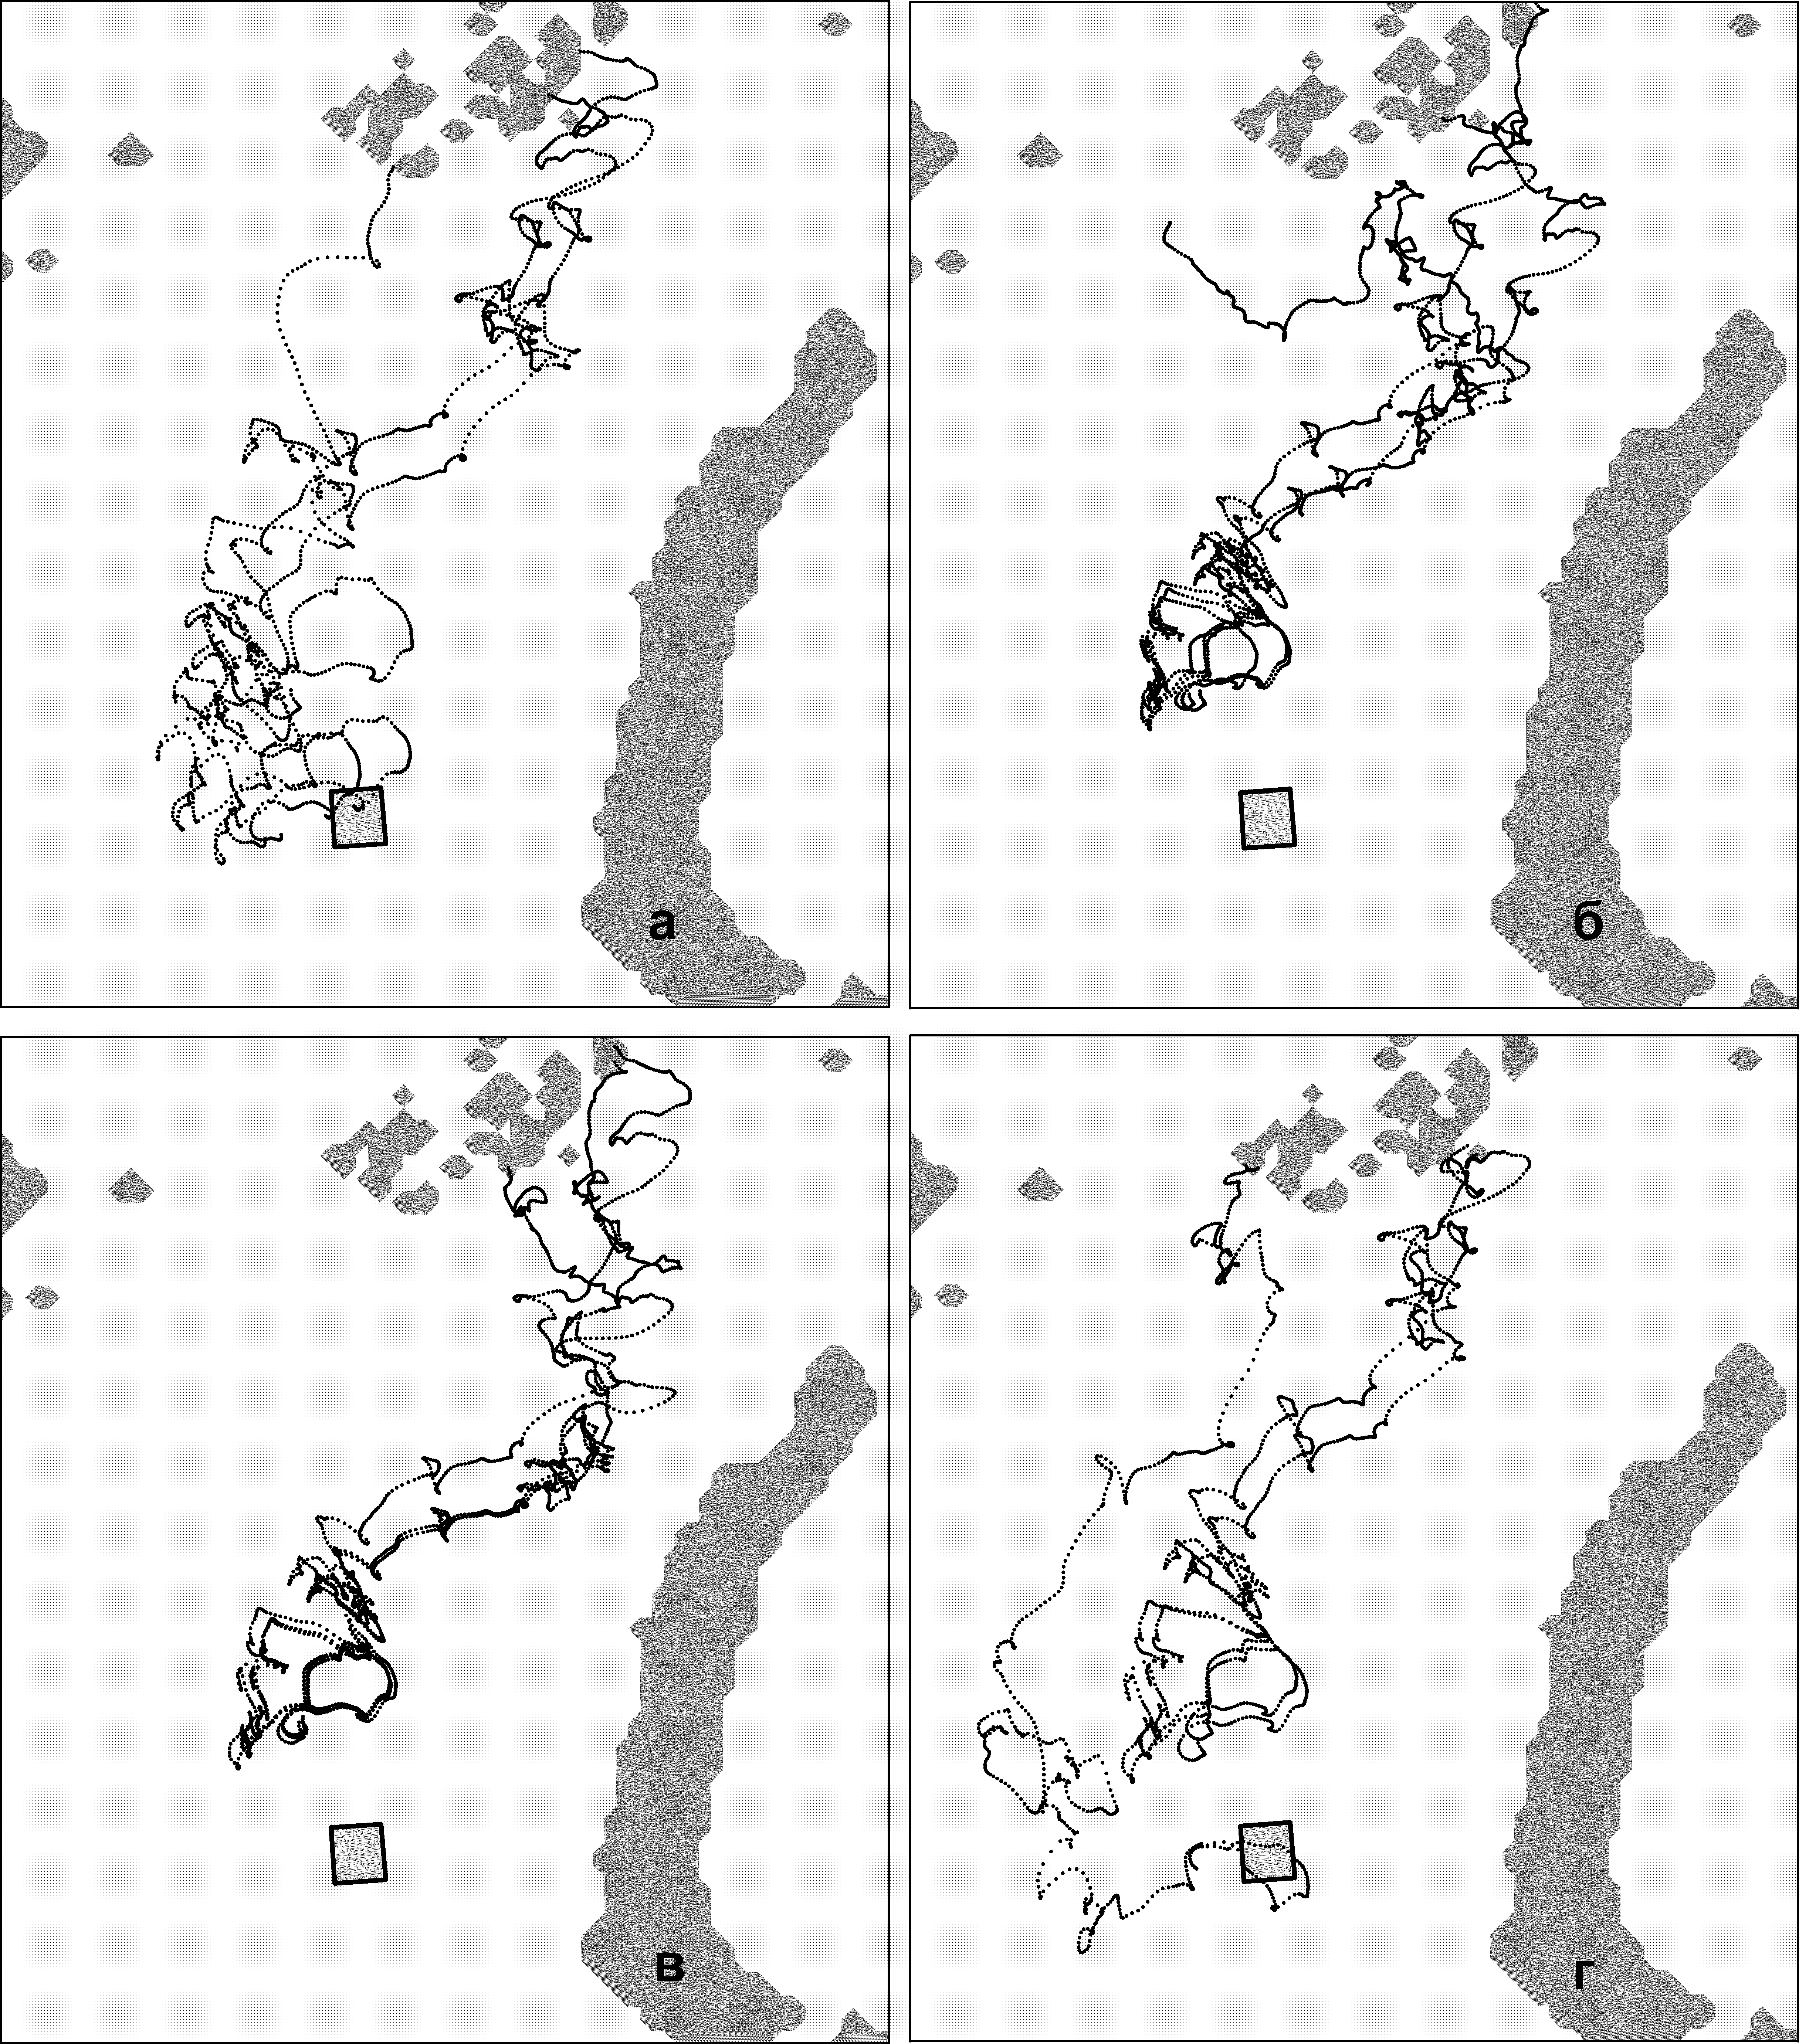
\includegraphics [scale=0.07] {ibg_frc_shtk}
	\caption{Рассчитанные траектории обратного дрейфа айсбергов в 2003"--~2002 гг. от района ШГКМ для категорий: менее 60 тыс.т (а), от 100 до 400 тыс.т (б), от 400 до 700 тыс.т. (в) и свыше 1 млн.т. (г).}
	\label{img:ibg_frc}
\end{figure}

Результаты продемонстрировали, что все айсберги, обнаруженные и измеренные в рамках экспедиции <<ШТОКМАН"~ЗИМА"~2003>> пришли в район ШГКМ от архипелага Земля Франца"~Иосифа. В первую очередь, следует отметить, что, несмотря на широкое многообразие морфометрических особенностей и масс айсбергов, большая часть их траекторий (9 из 12) закончилась у юго-восточного побережья архипелага, подтвердив тем самым предположение авторов~\cite{Buzin2008} о том, что наиболее вероятном источником айсбергов, могущих достигнуть район ШГКМ, является ледник на Земле Вильчека.

Время дрейфа айсбергов от побережья архипелага Земля Франца-Иосифа до района ШГКМ по результатам расчетов составило: для самого малого айсберга №1 "--- 5 месяцев, для остальных айсбергов "--- от 7 до 10 месяцев. Таким образом, наиболее благоприятным для достижения айсбергами района ШГКМ является период июль "--- октябрь. Не противоречит это и наблюдавшейся в 2002 г. ледовой обстановке вокруг архипелага Земля Франца"~Иосифа. В начале июля все южное побережье уже было свободно не только от дрейфующих льдов, но и от припая.

Таким образом, выполненные модельные эксперименты показали, что ледники архипелага Земля Франца"~Иосифа являются наиболее вероятным источником айсбергов, опасных для добывающей платформы на ШГКМ. Время достижения айсбергами района ШГКМ составляет от 7 до 10 месяцев, но возможно и более быстрое продвижение. Все это необходимо учитывать при разработке системы мониторинга айсбергов на акватории Баренцева моря.

\subsection{Выводы}\label{subsect4_1_4}
Разработана технология мониторинга дрейфа айсбергов на основе численной гидродинамической модели, с использованием данных автоматизированного анализа спутниковых SAR"~изображений, которая может использоваться для решения целого ряда задач в системе мониторинга ледовой обстановки в Западной Арктической зоне Российской Федерации. 

Оперативное применение модели для производства краткосрочных прогнозов (24"--~72 часа) для гидрометеорологического обеспечения разведочного бурения на геологической структуре «Университетская"~1» на лицензионном участке Восточно"~Приновоземельский"~1 в Карском море в 2014 г. продемонстрировало эффективность разработанной технологии. 

Численные эксперименты на модели позволили получить важные закономерности распространения айсбергов в Баренцевом море, которые будут востребованы при оптимизации системы мониторинга в Западной Арктике.


%\newpage
%============================================================================================================================

\section{Параграф - два} \label{sect4_2}

Некоторый текст.

%\newpage
%============================================================================================================================

\section{Параграф с подпараграфами} \label{sect4_3}

\subsection{Подпараграф - один} \label{subsect4_4_1}

Некоторый текст.

\subsection{Подпараграф - два} \label{subsect4_4_2}

Некоторый текст.

\clearpage           % Глава 4
\include{Dissertation/conclusion}      % Заключение
\chapter*{Список сокращений и условных обозначений}             % Заголовок
\addcontentsline{toc}{chapter}{Список сокращений и условных обозначений}  % Добавляем его в оглавление
\noindent
%\begin{longtabu} to \dimexpr \textwidth-5\tabcolsep {r X}
\begin{longtabu} to \textwidth {r X}
% Жирное начертание для математических символов может иметь
% дополнительный смысл, поэтому они приводятся как в тексте
% диссертации
$\begin{rcases}
a_n\\
b_n
\end{rcases}$  & 
\begin{minipage}{\linewidth}
коэффициенты разложения Ми в дальнем поле соответствующие
электрическим и магнитным мультиполям
\end{minipage}
\\
${\boldsymbol{\hat{\mathrm e}}}$ & единичный вектор \\
$E_0$ & амплитуда падающего поля\\
$\begin{rcases}
a_n\\
b_n
\end{rcases}$  & 
коэффициенты разложения Ми в дальнем поле соответствующие
электрическим и магнитным мультиполям ещё раз, но~без окружения
minipage нет вертикального выравнивания по~центру.
\\
$j$ & тип функции Бесселя\\
$k$ & волновой вектор падающей волны\\

$\begin{rcases}
a_n\\
b_n
\end{rcases}$  & 
\begin{minipage}{\linewidth}
\vspace{0.7em}
и снова коэффициенты разложения Ми в дальнем поле соответствующие
электрическим и магнитным мультиполям, теперь окружение minipage есть
и добавлено много текста, так что описание группы условных
обозначений значительно превысило высоту этой группы... Для отбивки
пришлось добавить дополнительные отступы.
\vspace{0.5em}
\end{minipage}
\\
$L$ & общее число слоёв\\
$l$ & номер слоя внутри стратифицированной сферы\\
$\lambda$ & длина волны электромагнитного излучения
в вакууме\\
$n$ & порядок мультиполя\\
$\begin{rcases}
{\mathbf{N}}_{e1n}^{(j)}&{\mathbf{N}}_{o1n}^{(j)}\\
{\mathbf{M}_{o1n}^{(j)}}&{\mathbf{M}_{e1n}^{(j)}}
\end{rcases}$  & сферические векторные гармоники\\
$\mu$  & магнитная проницаемость в вакууме\\
$r,\theta,\phi$ & полярные координаты\\
$\omega$ & частота падающей волны\\
  \textbf{SAR} & synthetic apperture radar, радар с синтезированной апертурой\\
  \textbf{BEM} & boundary element method, метод граничных элементов\\
  \textbf{CST MWS} & Computer Simulation Technology Microwave Studio
  программа для компьютерного моделирования уравнений Максвелла\\
  \textbf{DDA} & discrete dipole approximation, приближение дискретиных диполей\\
  \textbf{FDFD} & finite difference frequency domain, метод конечных
  разностей в~частотной области\\
\textbf{FDTD} & finite difference time domain, метод конечных
разностей во временной области\\
\textbf{FEM} & finite element method,  метод конечных элементов\\
\textbf{FIT} & finite integration technique, метод конечных интегралов\\
\textbf{FMM} & fast multipole method, быстрый метод многополюсника\\
\textbf{FVTD} & finite volume time-domain, метод конечных объёмов во
временной области\\
\textbf{MLFMA} & multilevel fast multipole algorithm, многоуровневый
быстрый алгоритм многополюсника\\
\textbf{MoM} & method of moments, метод моментов\\
\textbf{MSTM} & multiple sphere T-Matrix, метод Т-матриц для множества сфер\\
\textbf{PSTD} & pseudospectral time domain method, псевдоспектральный
метод во временной области \\
\textbf{TLM} & transmission line matrix method, метод матриц линий
передач\\

\end{longtabu}
\addtocounter{table}{-1}% Нужно откатить на единицу счетчик номеров таблиц, так как предыдующая таблица сделана для удобства представления информации по ГОСТ
        % Список сокращений и условных обозначений
\include{Dissertation/dictionary}      % Словарь терминов
\include{Dissertation/references}      % Список литературы
\include{Dissertation/lists}           % Списки таблиц и изображений (иллюстративный материал)
%\include{Dissertation/appendix}        % Приложения

\end{document}
